\documentclass[11pt]{book}
\usepackage{answers}

\usepackage{fullpage}
\usepackage{amsmath,amsfonts,amsthm,mathrsfs,mathpazo,xspace,hyperref,graphicx}
\usepackage{endnotes}
\usepackage{color}
\usepackage{bm}
\usepackage{times}
\usepackage{amssymb,latexsym}
\usepackage{enumitem}
\usepackage{tikz-cd}

\setlist[itemize]{itemsep=1pt, topsep=1pt}

\newtheorem{theorem}{Theorem}[chapter]
\newtheorem{assumption}{Assumption}
\newtheorem{proposition}[theorem]{Proposition}
\newtheorem{conjecture}[theorem]{Conjecture}
\newtheorem{lemma}[theorem]{Lemma}
\newtheorem{claim}[theorem]{Claim}
\newtheorem{fact}[theorem]{Fact}
\newtheorem{corollary}[theorem]{Corollary}

\theoremstyle{remark}
\newtheorem{remark}[theorem]{Remark}

\theoremstyle{definition}
\newtheorem{definition}[theorem]{Definition}
\newtheorem{example}[theorem]{Example}
\newtheorem{oq}[theorem]{Open Question}

\newcommand{\beq}{\begin{eqnarray}}
\newcommand{\eeq}{\end{eqnarray}}

\newcommand{\ket}[1]{|#1\rangle}
\newcommand{\bra}[1]{\langle#1|}
\newcommand{\proj}[1]{\ket{#1}\!\bra{#1}}
\newcommand{\Tr}{\mbox{\rm Tr}}
\newcommand{\Id}{\ensuremath{\mathop{\rm Id}\nolimits}}
\newcommand{\Es}[1]{\textsc{E}_{#1}}

\newcommand{\reg}[1]{{\textsf{#1}}}

\newcommand{\C}{\ensuremath{\mathbb{C}}}
\newcommand{\N}{\ensuremath{\mathbb{N}}}
\newcommand{\F}{\ensuremath{\mathbb{F}}}
\newcommand{\K}{\ensuremath{\mathbb{K}}}
\newcommand{\R}{\ensuremath{\mathbb{R}}}
\newcommand{\Z}{\ensuremath{\mathbb{Z}}}

\newcommand{\pq}{\mathfrak{Q}}
\newcommand{\pv}{\mathfrak{V}}


\newcommand{\mA}{\mathcal{A}}
\newcommand{\mB}{\mathcal{B}}
\newcommand{\mC}{\mathcal{C}}
\newcommand{\mF}{\mathcal{F}}
\newcommand{\mH}{\mathcal{H}}
\newcommand{\mP}{\mathcal{P}}
\newcommand{\mQ}{\mathcal{Q}}
\newcommand{\mS}{\mathcal{S}}
\newcommand{\mX}{\mathcal{X}}
\newcommand{\mY}{\mathcal{Y}}

\newcommand{\setft}[1]{\mathrm{#1}}
\newcommand{\State}{\setft{S}}
\newcommand{\Density}{\setft{D}}
\newcommand{\Pos}{\setft{Pos}}
\newcommand{\Proj}{\setft{Proj}}
\newcommand{\Channel}{\setft{C}}
\newcommand{\Unitary}{\setft{U}}
\newcommand{\Herm}{\setft{Herm}}
\newcommand{\Lin}{\setft{L}}
\newcommand{\Trans}{\setft{T}}
\DeclareMathOperator{\poly}{poly}
\DeclareMathOperator{\negl}{negl}

\newcommand{\eps}{\varepsilon}
\newcommand{\ph}{\ensuremath{\varphi}}

\newcommand{\BQP}{\textsc{BQP}}
\newcommand{\EXP}{\textsc{EXP}}
\newcommand{\BPP}{\textsc{BPP}}
\newcommand{\IP}{\textsc{IP}}
\newcommand{\QIP}{\textsc{QIP}}
\newcommand{\NP}{\textsc{NP}}
\newcommand{\PSPACE}{\textsc{PSPACE}}
\newcommand{\QMA}{\textsc{QMA}}
\newcommand{\NEXP}{\textsc{NEXP}}
\newcommand{\MIP}{\textsc{MIP}}
\newcommand{\QMIP}{\textsc{QMIP}}
\newcommand{\PCP}{\textsc{PCP}}
\newcommand{\RE}{\textsc{RE}}
\newcommand{\PP}{\textsc{PP}}
\newcommand{\PH}{\textsc{PH}}
\newcommand{\ALL}{\textsc{ALL}}
\newcommand{\QCMA}{\textsc{QCMA}}



\newcommand{\ol}[1]{\overline{#1}}

\newcommand{\tnote}[1]{\textcolor{magenta}{\small {\textbf{(Thomas:} #1\textbf{)
      }}}}
\newcommand{\com}[1]{\textcolor{blue}{\small {\textbf{(Comment:} #1\textbf{)
      }}}}
\newcommand{\typo}[1]{\textcolor{red}{\small {\textbf{(Typo:} #1\textbf{)
      }}}}
			
\bibliographystyle{alpha}

 

\renewcommand{\chaptername}{Lecture}
\newtheorem{exercise}{Exercise}[chapter]
\Newassociation{solution}{Soln}{mycor}
\renewcommand{\Solnlabel}[1]{\textbf{Answer #1}}

\title{Lecture notes on the Mahadev verification protocol\footnote{These lecture notes are based on four lectures given in October and November 2020 at the Institut Henri Poincar\'e (IHP) in Paris, under the sponsorship of the Fondation Sciences Math\'ematiques de Paris (FSMP). I thank the FSMP, the IHP, and the students in the course for feedback and corrections. A complete set of notes for the 10-week course is available at~\href{http://users.cms.caltech.edu/\~{}vidick/teaching/fsmp/fsmp.pdf}{http://users.cms.caltech.edu/~vidick/teaching/fsmp/fsmp.pdf}.}}
\author{Thomas Vidick}
%\includeonly{Lecture1}
%\includeonly{Lecture2}
%\includeonly{Lecture3}
%\includeonly{Lecture4}

\begin{document}

\maketitle





\tableofcontents

\chapter{Testing a qubit under computational assumptions}
\label{chap:computational-test}

The goal of these four lectures is to describe and analyze an interactive protocol that can be used to classically and efficiently certify  that a quantum device implements an entire quantum computation of one's choice. 

In the first lecture we introduce the main ideas of the protocol in an elementary setting by describing a ``computational test for a qubit,'' whose soundness rests on a cryptographic assumption. The resulting interactive test can be executed to certify that a device has quantum capabilities. 
In the second lecture we formally define the problem of \emph{delegating quantum computations} to an untrusted party and introduce a delegation protocol due to Fitzsimons and Morimae~\cite{morimae2016post} that involves quantum communication from the prover to the verifier. 
In the last two lectures we combine the Fitzsimons-Morimae protocol with the computational qubit test from the first lecture and a few additional ideas to obtain the classical delegation protocol due to Mahadev~\cite{mahadev2018classical}.  

\medskip

We assume basic familiarity with classical complexity theory (interactive proofs) and quantum computation. These four lectures are adapted from a 10-week course, and the interested reader may consult the full notes available at~\href{http://users.cms.caltech.edu/\~{}vidick/teaching/fsmp/fsmp.pdf}{http://users.cms.caltech.edu/~vidick/teaching/fsmp/fsmp.pdf} for background and a presentation of additional results related to the ones discussed here.

\section{Introduction}

Suppose given the possibility to interact with an arbitrary ``device'', or \emph{prover}, modeled as a black-box interactive machine. Suppose that the interaction is restricted to the exchange of classical messages, and that the \emph{verifier} executing the interaction is itself modeled as a classical probabilistic polynomial-time (PPT) machine. Can the PPT verifier implement a test that allows it to certify, with high confidence, that the behavior demonstrated by the device is quantum, i.e.\ it does not have a classical realization? 

In general this is not possible: almost by definition any input-output behavior has a classical model. An additional assumption thus needs to be introduced. In these lectures we consider the natural assumption that the device is itself a polynomial-time machine; however, it may implement arbitrary \emph{quantum} polynomial-time (QPT) computations. Our setting is thus that of a PPT verifier interacting with a QPT prover. 

A simple interactive ``test of quantumness'' in this setting consists in asking the device to factor a large integer $n$; under the assumption that factoring is hard for classical computers this test adequately distinguishes classical from quantum devices. 
The main limitation of this test that is generally pointed out is that in order for a device to successfully demonstrate its ``quantumness'' it needs to have the capability to implement a large, fault-tolerant quantum computation. If one's goal is solely to demonstrate quantumness then one may hope for a much simpler test, that could be implemented on a not-necessarily-universal quantum machine. Indeed, such tests have long been known under a different natural assumption of the prover, that it constitutes of two spatially isolated components.\footnote{See the full notes at~\href{http://users.cms.caltech.edu/\~{}vidick/teaching/fsmp/fsmp.pdf}{http://users.cms.caltech.edu/~vidick/teaching/fsmp/fsmp.pdf} for an in-depth discussion of this alternate model.} 

A second limitation that is relevant for us is that the factoring test does not seem to provide a means to certify anything beyond quantumness of the device. Crucially, it does not give us any handle on \emph{how} the device successfully passed the test. To build towards more interesting tests, such as a test for certifying randomness or even a complete quantum computation, we need to develop means that allow us to exert a greater control over the device's workspace: informally, we need to be able to certify that the device ``has some qubits'' and operates on them in a certain way. 

The goal of this lecture is to introduce a test of quantumness that has this feature: the test allows us to certify, in a precise sense, that any device that succeeds in it ``has a qubit''; moreover, we will gain a solid understanding of ``where'' that qubit ``is''. A key insight from the lecture is that in order to obtain such a  test we will need to assume that a certain problem is hard not only for classical computers (such as factoring) but also for quantum computers. We start with a definition of a qubit. 

\section{What is a qubit?}

The  ``qubit'' is generally introduced in quantum computing courses through its \emph{state space}, which is the set of unit vectors in the complex vector space $\C^2$; we denote this space as $\State(\C^2)$. Thus the \emph{state of a qubit} can be represented by a unit vector in $\C^2$; for example, 
\[\ket{0} = \begin{pmatrix} 1 \\ 0 \end{pmatrix}\qquad\text{and}\qquad \ket{+} = \frac{1}{\sqrt{2}}\begin{pmatrix} 1 \\ 1 \end{pmatrix}\]
are both valid states for a qubit. So we all know how to recognize a valid state for a qubit. But what about \emph{the qubit itself}? Consider an analogous formalization of the notion of a ``probabilistic bit'', a two-level system that can be in any ``superposition'' of its two states, $p \,\ol{0} + (1-p)\,\ol{1}$ for any $p\in [0,1]$. What distinguishes the real, ``$1$-dimensional'' degree of freedom $p\in [0,1]$  of the probabilistic bit from the complex, ``$2$-dimensional'' degree of freedom of the qubit?

To give a precise definition we turn to the ``Heisenberg representation'' of quantum mechanics, that places \emph{observable} quantities at a forefront. Informally, we will distinguish a quantum degree of freedom from a classical one by requiring that the quantum degree of freedom can be measured (observed) in two \emph{mutually incompatible ways}.  
Recall that in quantum mechanics an observable is specified by 
 a Hermitian operator $O$ on $\mH$.
 Each eigenvalue of $O$ represents a possible outcome under a measurement of the observable, and  the associated eigenvectors denote states under which the observable deterministically yields that outcome. 
An observable such that $O^2=\Id$ has at most two eigenvalues, $-1$ and $+1$. Such an observable is called a \emph{binary} observable; it is the most frequent kind of observable that we will encounter. 

\subsection{First definition of a qubit}

The following definition makes precise our informal presentation of a ``qubit'' as ``a system that can be observed in two mutually incompatible ways''. 

\begin{definition}[Qubit, Take 1]\label{def:qubit-take1}
A \emph{qubit} is a triple $(\mH,X,Z)$ consisting of a separable Hilbert space $\mH$ and a pair of Hermitian operators $X,Z$ acting on a $\mH$ such that $X^2=Z^2=\Id$ and $\{X,Z\}=XZ+ZX=0$.
\end{definition}

Let's see why 
Definition~\ref{def:qubit-take1} captures the intuitive notion of ``mutually incompatible'' observables. Let the 'computational basis' be an eigenbasis of $Z$, and the 'Hadamard basis' an eigenbasis of $X$. Then we claim that the anticommutation relation $XZ+ZX=0$ ensures that any vector in the former makes a $45^{\circ}$ angle with any vector in the latter. To see this, let $\ket{\psi}$ be an eigenvector of $X$ with associated eigenvalue $\eps\in\{\pm 1\}$. Then $\bra{\psi} XZ + ZX \ket{\psi} = 0$ immediately implies $2\eps\bra{\psi} Z \ket{\psi}=0$. Given that $Z$ only has $-1$ and $+1$ as eigenvalues, this relation implies that the projections of $\ket{\psi}$ on the two eigenspaces of $Z$ have equal length; in other words, $\ket{\psi}$ lies exactly between the $+1$ and $-1$ eigenspaces of $Z$. (Yet another way of saying this is that all principal angles between an eigenspace of $X$ and one of $Z$ are $\frac{\pi}{4}$.) In this sense any $X$ and $Z$ satisfying the conditions of the definition are ``maximally incompatible'': any definite state for the one is entirely undetermined (i.e.\ yields uniformly random outcomes when measured) under the other. 

There is a problem with this definition: by allowing the underlying Hilbert space $\mH$ to be arbitrary we seem to have all but lost the usual requirement that a qubit is a system whose state space is ``two-level'' and thus identifiable with the projective space $\State(\C^2)$. Luckily, the following lemma allows us to make the connection with this requirement. 

\begin{lemma}\label{lem:qubit-c2}
Let $(\mH,X,Z)$ be a qubit. Then there is a Hilbert space $\mH'$ and an isomorphism $\mH\simeq \C^2 \otimes \mH'$ such that under the same isomorphism, $X\simeq \sigma_X\otimes \Id$ and $Z\simeq \sigma_Z \otimes \Id$.\footnote{The reader might wonder what happened to $\sigma_Y$... Don't we need it to define our qubit? Here we are taking the ``operator algebraists''' perspective, which is that if the system supports $X$ and $Z$ observables then it also supports $Y=iXZ$. Because $Y$ is determined by $X$ and $Z$, we do not include it in the definition.} Here, $\sigma_X$ and $\sigma_Z$ are the usual Pauli observables on $\C^2$: in matrix form, 
\[ \sigma_X = \begin{pmatrix} 0 & 1 \\ 1 & 0 \end{pmatrix} \qquad\text{and}\qquad\sigma_Z = \begin{pmatrix} 1 & 0 \\ 0 & -1 \end{pmatrix}\;.\]
\end{lemma}

Note that a consequence of the lemma is that qubits, as defined in Definition~\ref{def:qubit-take1}, only exist in spaces of even (or infinite) dimension! In particular, qubits don't exist in dimension $1$; indeed, in dimension $1$ all operators commute. This is satisfactory: intuitively, a situation in which all possible observables commute ought to be considered ``classical'' (for instance, because there is a complete set of simultaneous eigenvectors for all observables). 

It will be essential for our later goals that Definition~\ref{def:qubit-take1} does not \emph{a priori} require $\mH$ to be a two-dimensional space. Indeed, how would one test such a claim? One does not ``see'' the dimension of the state space; while it is possible to probe parts of it it can never be excluded that the state space is larger than what is accessible to the experimentalist's setup. In this sense Definition~\ref{def:qubit-take1} has a nice ``operational'' flavor to it: it refers to \emph{observables} of the system and their properties.  Although much work is needed before we are able to make any of these statements formal, we see the definition as a good step towards giving us the ability to ``test'' that a system ``is a qubit''. In addition, the definition clearly has meaningful consequences; in particular it implies that qubits do not have a ``classical explanation'', so that a ``test for a qubit'' can serve as a ``test for quantumness'', i.e.\ a test that distinguishes quantum from classical behavior. 

The proof of the lemma makes use of an elementary but fundamental tool in the analysis of many quantum information protocols, the CS (for ``Cosine-Sine'') decomposition. We recommend the proof as an exercise to the reader.\footnote{For a solution, see the full notes~\href{http://users.cms.caltech.edu/\~{}vidick/teaching/fsmp/fsmp.pdf}{http://users.cms.caltech.edu/~vidick/teaching/fsmp/fsmp.pdf}.}

\subsection{A second definition}

Unfortunately Definition~\ref{def:qubit-take1} is impossible to ``test''. In any actual interaction with the device the only information available to the verifier is the result of the device's measurements \emph{when performed on its quantum state}. Requiring that the observables themselves anti-commute is too stringent: one may only hope to certify how the observables act \emph{on the state}, not in general. 

To make this point clear, consider the fist step in the analysis of any interactive protocol: how do we model the actions of an arbitrary prover? At each stage the prover receives a question $x\in \mX$ and is expected to provide an answer $a\in\mA$, where $\mX$ and $\mA$ are finite sets that are specified by the protocol. Under the assumption that the prover's actions can be modeled using quantum mechanics, which we will always make, there must exist a Hilbert space $\mH$  associated with the prover and a state $\rho \in \Density(\mH)$ that the prover possesses at the start of the protocol. (We use $\Density(\mH)$ to denote the set of all density matrices, i.e.\ positive semidefinite matrices of trace $1$, on $\mH$.)
When the prover receives its question $x$ it measures some observable $O_x = \sum_a \lambda_a \Pi^x_a$, where $\lambda_a$ are arbitrary and $\Pi^x_a$ projections that sum to identity. According to the Born rule, it obtains an answer distributed as $\Pr(a|x) = \Tr(\Pi^x_a \rho)$.
 Finally the quantum state $\rho$ of the prover gets updated as a function of the outcome obtained.\footnote{This formalization is fully general; in particular it can be used to model classical deterministic strategies by setting $\Pi^x_a = 1_{f(x)=a}$ where $f$ would be the function used by the prover to determine its answers. Similarly, randomized strategies can be represented by making use  of a totally mixed state $\rho = \sum_r p_r \proj{r}$, for some arbitrary distribution $\{p_r\}$, to capture the randomness.}
When the interaction is executed the only observable data that is accessible to the experimentalist is, at best, the probabilities $\Pr(a|x)$.\footnote{We write ``at best'' because the experimentalist does not get to see probabilities. Under the i.i.d.\ assumption it can sometimes estimate them to within an additive error. However, in the case where $\mA$ is a large alphabet it may be that all probabilities are exponentially small. This will be the case in some of the experiments that we describe.}
If $O$ is an observable, $\ket{\psi}$ a state on which it acts, and $U$ an arbitrary unitary,
\[ \bra{\psi} O \ket{\psi} =\bra{U\psi}  (UOU^\dagger) \ket{U\psi}\;.\]
Thus two models of the prover, using state $\ket{\psi}$ and observable $O$ or using state $U \ket{\psi}$ and observable $UOU^\dagger$, lead exactly to the same observed data. Our earlier definition of a qubit, by ignoring the role played by the state and imposing constraints on the operators themselves, violates this. This leads us to update our first definition as follows. 

\begin{definition}[Qubit, Take 2]\label{def:qubit-2}
A \emph{qubit} is a triple $(\ket{\psi},X,Z)$ such that $\ket{\psi} \in \State(\mH$), where $\mH$ is a separable Hilbert space left implicit in the notation, and $X$ and $Z$ are Hermitian operators on $\mH$ such that
\begin{equation}\label{eq:ac-state}
\{X,Z\}\ket{\psi} = 0\;.
\end{equation}
\end{definition}

Note that the definition still makes the requirement that  $X^2=Z^2=\Id$ as operators. This is because this requirement follows from the laws of quantum mechanics themselves; informally, it just means that each of $X$ and $Z$ has a spectral decomposition with two associated eigenprojections, i.e.\ they represent valid binary observables. 

At this point there are two important questions we should be asking: (i) Is this definition meanginful? With the anti-commutator weakened as in~\eqref{eq:ac-state}, does the definition still capture our intuitive notion of a qubit? (ii) We weakened the definition in an arbitrary-looking way by inserting a dependence on the state vector $\ket{\psi}$. Can we justify this, i.e.\ are we now able to develop protocols that test the definition? The following lemma provides an answer to the first question. 

\begin{lemma}\label{lem:qubit-2-rigid}
Let $(\ket{\psi},X,Z)$  be a qubit on $\mH$. Then there exists a Hilbert space $\mH'$ and an isometry $V: \mH\to  \C^2 \otimes \mH'$  such that 
\begin{equation}\label{eq:qubit-2-rigid-a}
 V X \ket{\psi} =  (\sigma_X \otimes \Id )V \ket{\psi}\qquad \text{and}\qquad  V Z \ket{\psi} =  (\sigma_Z \otimes \Id )V \ket{\psi} \;.
\end{equation}
\end{lemma}

The following diagram illustrates the situation guaranteed by the lemma:
\begin{equation}\label{diag:one-qubit}
\begin{tikzcd}
\mH \arrow{r}{V} \arrow[swap]{d}{X,\; Z} & \C^2 \otimes \mH' \arrow{d}{\sigma_X\otimes \Id,\; \sigma_Z\otimes \Id} \\
\mH \arrow{r}{V} & \C^2 \otimes \mH'
\end{tikzcd}
\end{equation}
Note that the lemma no longer says that $X$ is \emph{equal} to $\sigma_X \otimes \Id$ (under the isomprhism $\pi$), but only that \emph{it has the same action on the state}, up to the isometry $V$. In particular, it is now possible for $\mH$ to have odd dimension. This is necessary: for example, we can set
\[ \ket{\psi} = \begin{pmatrix} 1 \\ 0 \\ 0 \end{pmatrix}\;,\quad X = \begin{pmatrix} 0 & 1 & 0 \\ 1 & 0 & 0 \\ 0 & 0 & 1 \end{pmatrix}\;,\quad Z =  \begin{pmatrix} 1 & 0 & 0 \\ 0 & -1 & 0 \\ 0 & 0 & 1 \end{pmatrix}\]
and still satisfy Definition~\ref{def:qubit-2}.  Here, the third dimension has been added to the operators but since none of $\ket{\psi}$, $X\ket{\psi}$ or $Z\ket{\psi}$ has support on it it is ``inaccessible'' to any experiment that involves only this state and operators. However, it is good to verify that the definition is non-trivial, and in particular requires $\dim(\mH)\geq 2$. Indeed, suppose that $X\ket{\psi}$ and $Z\ket{\psi}$ are colinear. Then by~\eqref{eq:qubit-2-rigid-a} it follows that $(\sigma_X\otimes \Id)V\ket{\psi}$ and $(\sigma_Z\otimes \Id)V\ket{\psi}$ are colinear. As we saw in the previous lecture, due to $\{\sigma_X,\sigma_Z\}=0$ this is impossible. 

The proof of the lemma again follows from Jordan's lemma. In the third lecture we will see an explicit definition for the isometry $V$ that provides an alternate proof. For the remainder of the lecture we focus on the second question: can Definition~\ref{def:qubit-2} be tested in an interactive experiment? 

\begin{remark}
Definition~\ref{def:qubit-2} requires the anti-commutator $\{X,Z\}$ to be exactly zero when evaluated on the state $\ket{\psi}$. In general with any finite test we may only hope to characterize an ``approximate qubit'', which is defined as a triple $(\ket{\psi},Z,X)$ such that $\|\{X,Z\}\ket{\psi}\|\leq \eps$ for some $\eps\geq 0$ that measures the ``quality'' of the qubit. For convenience in these notes we often make a simplifying assumption of ``perfect success'' that allows us to achieve $\eps=0$; unless otherwise noted the statements and proofs that we give  extend readily to the general case.
\end{remark}

\section{Simon's algorithm}

Having defined the object that we aim to certify, we now remind ourselves of the tools at our disposition by reviewing the prototypical example of a task for which the manipulation of quantum information provides  a computational advantage.

\subsection{The algorithm}
\label{sec:simon-algorithm}

The input to an instance of Simon's problem is a function $f:\{0,1\}^n\to \{0,1\}^n$ that has the property that $f$ is $2$-to-$1$ (every value in the range has exactly two preimages) and moreover there is a string $s\in\{0,1\}^n$ such that for every $x,y\in\{0,1\}^n$, $f(x)=f(y)$ if and only if $y=x$ or $y=x+ s$, where addition is performed coordinate-wise and modulo $2$. The goal is to recover the string $s$. It is not hard to see that in the worst case any classical algorithm requires at least $\Omega(2^{n/2})$ evaluations of $f$ to determine $s$. This is because on the one hand for any deterministic algorithm that makes a smaller number of evaluations there is a function $f$ such that all values returned by $f$ are distinct, so no information about $s$ is gained; similarly one can show that for any randomized algorithm if $f$ is chosen at random then it is unlikely that the algorithm will gain any information about $s$ in $\ll 2^{n/2}$ evaluations. On the other hand, by making roughly $\Omega(2^{n/2})$ evaluations at random points then by the birthday paradox one will likely obtain $x\neq y$ such that $f(x)=f(y)$, which immediately reveals $s=x+ y$. 

Simon showed that there is a quantum algorithm that can solve this problem using only $O(n)$ evaluations, provided that the function $f$ can be evaluated ``in superposition''. The algorithm first evaluates $f$ on a uniform superposition of inputs, as follows:
\begin{align*}
\ket{0^n}\ket{0^n} & \mapsto \frac{1}{\sqrt{2^n}}\sum_x \ket{x} \ket{0^n}\notag\\
&\mapsto  \frac{1}{\sqrt{2^n}} \sum_x \ket{x} \ket{f(x)}\notag\;.
\end{align*}
It then measures the last register in the computational basis, yielding some $y=f(x_0)=f(x_1)$ where $x_0$ and $x_1 = x_0+ s$ are the two preimages of $y$ under $f$. The re-normalized post-measurement state is
\begin{equation}
 \frac{1}{\sqrt{2}}\big(\ket{x_0} + \ket{x_1}\big) \ket{y}\;. \label{eq:simon-1}
\end{equation}
Measuring the first register in the Hadamard basis yields a uniformly random $d\in\{0,1\}^n$ such that $d\cdot s = 0$. Repeating the entire procedure $O(n)$ times yields $(n-1)$ linearly independent such $d$'s, which suffices to recover $s$ with high probability. 


\subsection{Instantiating the black box}
\label{sec:simon-instantiate}

The main limitation of Simon's problem is that it only provides a \emph{black-box} separation: the quantum advantage holds under the assumption that the classical or quantum algorithms are allowed to evaluate the function $f$, but they are not given an explicit description of it. Showing that the separation still holds for an explicit choice of the function $f$ is much harder, because it is difficult to rule out some smart behavior for the classical algorithm that would take advantage of specific code for $f$; indeed, showing such a separation would be a major breakthrough in quantum algorithms. 

This difficulty shouldn't prevent us from toying with the question: Can we identify natural candidates? For example one could take $f(x) = Ax$ for $A\in \F_2^{n\times n}$ a matrix of rank exactly $(n-1)$. In that case the kernel of $A$ is spanned by a single vector $s\in\F_2^n$, and $f$ is exactly $2$-to-$1$: $f(x_0)=f(x_1)$ if and only if $A(x_0-x_1)=0$, i.e. $x_0-x_1$ is either $0$ or $s$. 
Unfortunately this $f$ is not a good candidate, because there happens to be an efficient classical algorithm that directly solves Simon's problem for it: Gaussian elimination.\footnote{In the last lecture we will see that a ``noisy'' version of $f$ provides a partial workaround.} The example shows that at a minimum we need a function $f$ that is $2$-to-$1$ but such that finding any colliding pair of inputs $(x_0,x_1)$ with $f(x_0)=f(x_1)$ is computationally difficult. In the next section we introduce some background from cryptography that will allow us to make this requirement precise. 

\section{Computational assumptions}

In this section we briefly review the formalism for making computational assumptions precise and apply it to a specific scenario  of interest for the lecture. 

\subsection{PPT and QPT procedures}

The first thing that we need to make precise is our computational model. Since the protocols we consider involve interaction between a verifier and prover we focus on modeling such devices as machines that perform a computation. Loosely speaking, each device operates in a number of rounds where at each round the device performs a computation that takes it from a certain internal state as well as an input (a message received from another device) to a new internal state and an output (a message that it returns). We will model each such computation as a circuit. A circuit is a sequence of elementary operations called ``gates'' that operate either on a classical state (in which case the gates can be things like an AND, an OR, a NOT, etc.) or a quantum state (in which case the gates can be things like a $1$-qubit Hadamard, a $\sigma_X$ or $\sigma_Z$, a $2$-qubit controlled NOT, etc.).\footnote{To be fully precise we would need to fix a finite gate set for classical circuits and another for quantum circuits. What gate set is used will not matter for us; the only important point is that there exists finite universal gate sets and that all such gate sets are roughly equivalent in terms of how many gates are required to decompose any larger unitary.} To recap, for us a verifier or a prover is specified by a sequence of classical or quantum circuits. We will always assume that the circuits explicitly specify which spaces they are meant to operate on (e.g. verifier's space, message from verifier to prover, etc.). 

Next we discuss what it means for a verifier (or prover) to be ``efficient''. To make this precise we need to talk about \emph{families} of verifiers. We will imagine that there is an underlying size parameter $n\in \N$ (for example, $n$ could be the size of a $3$SAT formula that the verifier aims to check, or the number of qubits that she aims to certify) and that the verifier (or prover) is specified by a classical Turing machine $M$ that on input $1^n$ returns an explicit classical description of a sequence of circuits that can be used to implement the verifier (or prover) for problems of size $n$. We will say that the verifier (or prover) is \emph{probabilistic polynomial time} (PPT) (resp. \emph{quantum polynomial time} (QPT)) if this Turing machine runs in time polynomial in its input (i.e.\ polynomial in $n$; this is why we always assume that $n$ is passed in unary to $M$) and returns a family of classical (resp. quantum) circuits. Note that the assumption that the Turing machine is polynomial time immediately implies that the circuits it returns act on polynomially many bits (resp. qubits) and have a polynomial number of classical (resp. quantum) gates. 

In a cryptographic context we will generally allow $M$ to take a second input $1^\lambda$ for $\lambda\in \N$ called the \emph{security parameter}. While the input size $n$ is governed by the size of the problem, the security parameter can be chosen at will; the larger it is the more ``secure'' the protocol is supposed to be (for example, the smaller the probability that the verifier makes an incorrect decision or the higher the quality of the certified qubits). 

\subsection{Claw-free functions}

Similarly to circuits in the previous section, when we talk about computational \emph{difficulty} of a certain problem we always need to refer to \emph{families} of objects. This is because e.g. for any given function $f$ there is nothing ``hard'' about the task of recovering specific information about $f$: if $f$ is fixed everything about it is fixed as well; in particular in the case when $f$ has the periodic structure required for Simon's problem there is a simple algorithm that identifies $s$, and this is the algorithm that writes $s$ down starting from any initial state. 

For this reason we will always consider families of functions $\{f_{pk}: \{0,1\}^{m(\lambda)} \to \{0,1\}^{m(\lambda)}\}_{pk\in\{0,1\}^{k(\lambda)}}$ where the index $\lambda \in \mathbb{N}$ is called \emph{security parameter} and $k$ and $m$ are polynomially bounded functions of $\lambda$; the idea is that for each $\lambda$ there is a collection of functions, indexed by strings of length $k(\lambda)$ and with the same domain and range, such that the larger the $\lambda$ the more ``complex'' the functions are. For example, we could take $k(\lambda)=\lambda^2$, $m(\lambda)=\lambda$, and $f_{pk}$ to be multiplication by the matrix $A\in\{0,1\}^{\lambda\times \lambda}$ obtained by ``reshaping'' the $\lambda^2$-bit string $pk$ into a $\lambda\times\lambda$ square. 

Let's give our first definition of a cryptographic property that applies to a family of functions. 

\begin{definition}[Claw-free function family]
A family $\mF = \{f_{pk}: \{0,1\}^{m(\lambda)} \to \{0,1\}^{m(\lambda)}\}_{pk\in\{0,1\}^{k(\lambda)}}$ is \emph{claw-free} against classical (resp. quantum) adversaries if 
the following conditions hold:
\begin{itemize}
\item $f_{pk}$ can be efficiently evaluated: there is a PPT procedure that given $pk$ and $x$ as inputs returns $f_{pk}(x)$.
\item For every $\lambda\in \mathbb{N}$ and  $pk\in\{0,1\}^{k(\lambda)}$, $f_{pk}$ is $2$-to-$1$.
\item For every PPT (resp. QPT) procedure $\mA$ the following holds: (the procedure $\mA$ is often personified as the ``adversary'' trying to demonstrate that the function family is \emph{not} claw-free) there exists a negligible\footnote{A function $\mu:\N\to\R$ is called {negligible} if for every polynomial $p$, $p(\lambda)\mu(\lambda)\to_{\lambda\to\infty} 0$.} function $\mu:\N\to\N$ such that for every $\lambda$, 
\[ \Pr_{pk\leftarrow_R \{0,1\}^{k(\lambda)}}\big( (x_0,x_1)\leftarrow \mA(1^\lambda,pk):\; x_0\neq x_1,\; f_{pk}(x_0)= f_{pk}(x_1)\big) \,\leq\, \mu(\lambda)\;.\]
\end{itemize}
\end{definition}

In words, the third condition states that there is no polynomial-time algorithm that given a uniformly chosen index $pk$ for a function from the family is able to return two distinct inputs for the function that constitute a claw.\footnote{A triple $(x_0,x_1,y)$ such that $x_0\neq x_1$ and $f(x_0)=f(x_1)=y$ is called a \emph{claw}. To see why, picture the arrows $x_0\rightarrow y$ and $x_1\rightarrow y$ drawn with $x_0,x_1$ on top of each other on the left and $y$ on the right.}

\begin{remark}
In the definition we require the function family to be parametrized by arbitrary strings $pk$. In general this requirement can be relaxed; in fact there could even be a single function for every $\lambda$. In cryptographic constructions the function family generally comes equipped with a PPT \emph{key generation procedure} $\textsc{Gen}$ that takes $1^\lambda$ as input and returns $pk$.
\end{remark}

An example of a claw-free family of functions against PPT adversaries can be constructed as follows. (This construction appears in~\cite{goldwasser1985paradoxical}, where it is used to construct a digital signature scheme.) Let $N=pq$ be a product of two primes $p\equiv 3 \bmod 8 $ and $q\equiv 7 \bmod 8$. This choice ensures that $-1$ and $2$ are not squares $\bmod N$; moreover, if $Q_N$ denotes the set of quadratic residues (i.e.\ squares) modulo $N$ then $f_0(x)=x^2 \bmod N$ and $f_1(x)=4x^2 \bmod N$ are both permutations of $Q_N$. (This fact requires proof but it is a simple exercise in arithmetic.) However, suppose given a claw $(x_0,x_1)$ such that $x_0,x_1\in Q_N$ and $f_0(x_0)=f_1(x_1)$. Then $x_0^2 = 4 x_1^2$ but $x_0 \neq \pm 2x_1 \bmod N$ because $\pm 2x_1\notin Q_N$. Thus computing the GCD of $N$ with $x_0\pm 2x_1$ recovers a nontrivial factor. 

While this family of functions is claw-free with respect to PPT adversaries, it is clearly not claw-free against QPT adversaries, that can use Shor's algorithm to factor efficiently. We will construct such a function family in the next lecture; for the time being we assume its existence. 


\subsection{Hardcore bits}

Following the initial steps of Simon's algorithm as described in Section~\ref{sec:simon-algorithm} when instantiated with any $2$-to-$1$ function enables a quantum device to generate strings $d\in\{0,1\}^m$ such that $d\cdot (x_0 + x_1) = 0$, where $(x_0,x_1)$ are preimages of some $y\in \F_2^m$ by $f$. Intuitively one might expect that this represents a computational advantage, because $d$ provides an equation in $x_0+x_1$, which is some information about both preimages together. For example in the case where $x_0+ x_1 = s$, where $s$ is some fixed secret independent of $y$, we saw that provided the equation $d$ can be assumed to be uniformly distributed among all valid equations in $s$ then running the procedure $O(m)$ times gives sufficiently many equations to recover $s$. 

Unfortunately, as discussed in Section~\ref{sec:simon-instantiate} for the only function that we could think of that has this property it is in fact easy to recover $s$, even for a classical computer. This suggests that in general the assumption that $f$ satisfies the structure required for Simon's algorithm might be too strong to obtain an explicit candidate. Moreover, recall that at the start of the lecture we pointed out that our goal is not directly to find a task for which there is a quantum computational advantage, but instead we are trying to identify \emph{two} tasks that the quantum device can perform \emph{separately} but not \emph{simultaneously}---if someone, such as a classical device, was able to execute both tasks simultaneously then it would break the computational assumption. What could those two tasks be here? 

Starting from the state~\eqref{eq:simon-1} it is natural to measure in the Hadamard basis, obtaining as before an equation $d$ such that $d\cdot(x_0+ x_1)=0$, but also in the computational basis, obtaining either $x_0$ or $x_1$. Given that ``honest'' measurements in the computational and hadamard basis are incompatible, these are natural candidates for our ``qubit.'' However, we also saw that if $x_0+ x_1 = s$ for some fixed secret $s$ then the Hadamard measurements alone allow us to recover $s$. So a quantum procedure could recover $s$ ``on the side'' and then, knowing $f$ explicitly, succeed in any reasonable ``test'' by using classical operations alone---this would make it very hard for us to identify the ``qubit'' that the device should have used to recover $s$ (this is similar to the example of Shor's algorithm given at the start of the lecture). But what if the structure of $f$ is a little more complicated, so that e.g.\ $x_0 + x_1 = g(x_0,s)$ for some function $g$? In that case a single equation in $g(x_0,s)$ might not be so useful; even many such equations for varying $x_0$ could be useless since without knowledge of $x_0$ itself one cannot determine what the equation is about. However, if one was able to obtain $x_0$ simultaneously with the equation then one would obtain a sequence of (possibly non-linear, depending on $g$) constraints on $s$. These considerations motivate the following computational assumption:

\begin{assumption}[Adaptive hardcore bit]\label{ass:hc-bit}
There is a claw-free family of functions $\mF = \{f_{pk}\}$ such that  for any QPT adversary $\mA$ there is a negligible function $\mu$ such that 
\begin{equation}\label{eq:hc-bit-0}
\Big|\frac{1}{2} -  \Pr_{pk\leftarrow_R \{0,1\}^{k(\lambda)}}\Big( (x,d)\leftarrow \mA(1^\lambda,pk),\, \{x_0,x_1\}\leftarrow f_{pk}^{-1}(f_{pk}(x)):\; d\neq 0^m \wedge d\cdot ( x_0+x_1) = 0\Big)\Big| \,\leq\, \mu(\lambda)\;.
\end{equation}
\end{assumption}

In words, the assumption is that no \emph{quantum} polynomial-time algorithm can \emph{simultaneously} return an element $x$ in the domain of $f$ and an equation $d$ such that, letting $\{x_0,x_1\}$ be the two preimages of $f_{pk}(x)$ under $f_{pk}$ it holds that $d\neq 0^m$ and $d\cdot (x_0+x_1)=0$. Note that although we required $\{f_{pk}\}$ to be claw-free, this requirement is stronger, since any algorithm that can find a claw $(x_0,x_1)$ can be used to break~\eqref{eq:hc-bit-0}.

\begin{remark}
Assumption~\ref{ass:hc-bit} is called \emph{adaptive hardcore bit} for the following reason. Given a function $f$ a hardcore bit for $f$ is a $1$-bit function $h$ such that given $f(x)$ (but not $x$) it is hard to predict $h(x)$. Here, the hardcore bit that underlies the assumption is the function $h(x)=d\cdot (x_0+x_1)$ for any $d\neq 0^m$: the Goldreich-Levin theorem implies that if $f$ is indeed claw-free then it is hard to predict $b(x)$ for a \emph{random} $d$. The ``adaptive'' qualifier refers to the fact that in~\eqref{eq:hc-bit-0} we allow the adversary $\mA$ itself to select the equation $d$ without requiring that this equation is uniformly distributed  (we will see why this is needed in the next section); in particular $\mA$ may return always the same $d$, and this invalidates the classic Golreich-Levin argument. This makes the property harder to satisfy, because more power is given to the adversary. (Note in particular that we had to explicitly require $d\neq 0^m$, as otherwise there is an easy adversary that always succeeds.)
\end{remark}

\section{A computational test for a qubit}
\label{sec:comp-test}

We conclude the lecture by giving a ``proof of concept'' that it is possible to test a qubit based on computational assumptions. Our presentation is a simplified version of the protocol and analysis from~\cite{brakerski2018cryptographic}. For a related approach, see~\cite{cojocaru2019qfactory}. Recalling Definition~\ref{def:qubit-2}, in order to do this we will have to demonstrate that any device successful in the protocol ``has'' (in a sense that will be made precise in the proof) two observables 
 $X$ and $Z$ that are mutually incompatible. This incompatibility will be based on considerations of computational difficulty. Specifically we will show that, if the quantum device was able to measure $X$ and $Z$ jointly then it would  break a computational problem that is assumed to be hard \emph{even for quantum computers} --- this is as a form of ``computational uncertainty principle''. Since by definition the device can measure $X$ and $Z$ separately, if they commuted then it could also measure them jointly. Therefore, the computational assumption gives rise to an \emph{information-theoretic} consequence on the observables $X$ and $Z$: they must form a qubit.  

 The main computational assumption that we make is the existence of a function family $\{f_{pk}\}$ that satisfies the hardcore bit assumption, Assumption~\ref{ass:hc-bit}. In fact we will need a little bit more. Let's summarize the requirements as follows:
\begin{enumerate}[label=(\textbf{F.\arabic*})]
\item\label{ass:f1} There is a $2$-to-$1$ claw-free function family $\mF = \{f_{pk}\}$ equipped with an efficient key generation procedure $\textsc{Gen}(1^\lambda)$ such that for each key $pk$ the function $f_{pk}$ can be evaluated efficiently.
\item \label{ass:f2}The function family $\mF$ satisfies the adaptive hardcore bit assumption, Assumption~\ref{ass:hc-bit}.
\item\label{ass:f3} $\mF$ is equipped with a trapdoor: in addition to $pk$, $\textsc{Gen}(1^\lambda)$ returns a trapdoor $td$ such that given $pk$, $td$ and any $y$ in the range of $f_{pk}$ it is possible to efficiently recover the two preimages $x_0$ and $x_1$ of $y$. 
\item\label{ass:f4} For any $pk$ and any $y$ in the range of $f_{pk}$ the two preimages of $y$ are labelled '$x_0$' and '$x_1$' using some canonical efficient procedure. That is, given a key $pk$ and an $x$ in the domain of $f_{pk}$ it is possible to efficiently determine if $x$ is the '$x_0$' or the '$x_1$' preimage of $y=f(x)$. Let $b:\{0,1\}^m \to \{0,1\}$ be this labeling procedure; $b$ may depend on $pk$. 
\end{enumerate}
Let us fix a function family $\mF$ satisfying the assumptions~\ref{ass:f1} to~\ref{ass:f4}. We give a protocol based on $\mF$. The protocol describes the interaction between a classical polynomial-time verifier and a (possibly quantum) polynomial-time prover. Here, the input to both parties is the security parameter $\lambda$; when we refer to PPT or QPT we mean with respect to $\lambda$. The protocol is described in Figure~\ref{fig:protocol-comp-test}. For future reference we refer to it as ``protocol $\pq$.''

\begin{figure}[htbp]
\rule[1ex]{16.5cm}{0.5pt}\\
Let $\mF$ be a function family and $\lambda\in\mathbb{N}$ a security parameter. \begin{enumerate}
\item The verifier generates $(pk,td)\leftarrow \textsc{Gen}(1^\lambda)$. It sends $pk$ to the prover. 
\item The prover returns $y \in \{0,1\}^m$, where $m=m(\lambda)$. 
\item The verifier selects a uniformly random challenge $c\leftarrow_R \{0,1\}$ and sends $c$ to the prover. 
\item 
\begin{enumerate}
\item \emph{(pre-image test:)} In case $c=0$ the prover is expected to return an $x\in\{0,1\}^m$. The verifier accepts if and only if $f(x)=1$. 
\item \emph{(equation test:)} In case $c=1$ the prover is expected to return a $d\in \{0,1\}^m$. The verifier uses $td$ to determine the two preimages $(x_0,x_1)$ of $y$ by $f_{pk}$. She accepts if and only if $d\cdot(x_0+ x_1)=0$. 
\end{enumerate}
\end{enumerate}
\rule[1ex]{16.5cm}{0.5pt}
\caption{Protocol $\pq$, the computational test for a qubit. The protocol is parametrized by a function family~$\mF$ satisfying assumptions~\ref{ass:f1} to~\ref{ass:f4}.}
\label{fig:protocol-comp-test}
\end{figure}



\begin{theorem}\label{thm:comp-qubit}
Let $\mF$ satisfy the assumptions~\ref{ass:f1} to~\ref{ass:f4}. Then the following hold for protocol~$\pq$.
\begin{itemize}
\item (Completeness:) There is a QPT prover $P$ which succeeds with probability $1$ in the protocol.
\item (Soundness:) Suppose that a QPT prover $P$ succeeds with probability $1$ in the protocol. Then $P$ has a (near-perfect) qubit. 
\end{itemize}
\end{theorem}

We note the slightly informal nature of the theorem and make a few comments:
\begin{itemize}
\item Combining Assumption~\ref{ass:hc-bit} with the requirement that the prover $P$ is QPT effectively means that we are assuming that $P$ does not ``have the ability'' to violate~\eqref{eq:hc-bit-0}. Slightly more formally, in the proof we will show that if $P$ \emph{does not} ``have a qubit'' then it can be used to construct an adversary $\mA$ that violates~\eqref{eq:hc-bit-0}. Note also that in the soundness case it should be assumed that $P$ is in fact a family of $\{P_\lambda\}$, one for each possible choice of $\lambda$, that can be uniformly generated from $\lambda$ (i.e.\ there is a classical Turing machine that takes $1^\lambda$ as input and returns a description of a family of circuits that can be used to implement $P_\lambda$).\footnote{Non-uniform adversaries are allowed as long as we make the corresponding non-uniform cryptographic assumption.} 
\item
Second, we ought to be a little more precise as to how $P$'s qubit is specified. The two observables $X$ and $Z$ that define it will be derived from the two measurements that $P$ makes based on the challenges $c=0$ or $c=1$. Since these measurements in general have outcomes in $\{0,1\}^n$ some post-processing will be required. Interestingly, the post-processing for the $X$ observable will not be efficient, in the sense that it will require knowledge of $td$. So, our proof will show that there exists two anti-commuting observables on the Hilbert space of $P$ that can be defined from $P$'s operations \emph{and some classical post-processing}. Since the post-processing is classical we can claim in good faith that the ``qubit'' is located on the prover's space, as we are not injecting any external ``quantumness'' in it. 
\item
Regarding the assumption that the prover succeeds with probability $1$: this assumption is, of course, unrealistic. The assumption can be lifted at the cost of some amount of work, which we discuss in more detail when we build on the present protocol to construct a more complex protocol for verifying an entire quantum computation in the next lectures. 
\item
Finally, an explanation is in order regarding the ``(near-perfect)'' qualifier. This is an unavoidable consequence of the fact that the protocol relies on a computational assumption. Indeed, consider the following possible behavior for the prover. The prover first devotes a small amount of time to trying their luck at breaking the underlying computational assumption (in our case, the prover could randomly generate candidate trapdoors $td'$ and check if they allow it to invert the function $f_{pk}$). If the prover succeeds then it can pass in the protocol without manipulating any quantum state, using the fake $td'$ to find a claw that allows it to answer both types of challenges. If it does not succeed then it behaves honestly in the protocol. Such a prover succeeds with probability $1$, but the measurement operators associated with its answers have a part that is ``classical'' and from which we have no hope of extracting a qubit. 
\end{itemize}

\begin{proof}[Proof of Theorem~\ref{thm:comp-qubit}]
The completeness part of the theorem is clear. In the first phase the prover proceeds exactly as in Simon's algorithm to obtain the state~\eqref{eq:simon-1}. In the second phase, it measures the preimage register in the standard basis in case $c=0$ and in the Hadamard basis in case $c=1$, returning the $n$-bit outcome obtained as its answer. This prover is always accepted with probability $1$ in the protocol. 

To show the soundness part of the theorem we start with the usual (and, here, crucial) modeling step. 

\paragraph{Step 1: Modeling.} Since we will not need to model the prover's actions in the  first phase of the protocol in detail we directly give a name to the state of the prover at the end of step 2; let it be $\ket{\psi} \in  \mH_{\reg{P}}$. This state depends on $pk$ as well as on $y$; for clarity we suppress this dependence from the notation. Moreover, in general $\ket{\psi}$ may be a mixed state, and we represent it as a pure state for convenience only; in general one could assume that we included a register $\reg{E}$ to denote an ``environment'' that holds a purification $\ket{\psi}_{\reg{PE}}$ of a general $\rho \in \Density(\mH_{\reg{P}})$. 

At the second stage of the protocol the prover is given a challenge $c\in\{0,1\}$ and tasked with responding with an $n$-bit string, $x$ or $d$ depending on the challenge. In general, $x$ is obtained by performing a POVM $\{\Pi_x\}$ on the prover's entire space, and similarly $d$ is the outcome of a POVM $\{M_d\}$.\footnote{We do not need to explicitly mark any dependence of $\Pi$ or $M$ on $pk$ and $y$, because without loss of generality the prover has kept a classical copy of these strings in its quantum state $\ket{\psi}$, which can be used as a classical control by both $\Pi$ and $M$.} We make the following observations that allow us to simplify the presentation of these POVM:
\begin{itemize}
\item Without loss of generality both $\Pi$ and $M$ are projective measurements. This is because we can enlarge $\reg{P}$ and add sufficiently many ancilla qubits initialized to $\ket{0}$ so as to apply Naimark's theorem. 
\item Without loss of generality, assume that the prover has access to an $m$-qubit register $\reg{X}$ initialized to $\ket{0^m}$. 
\item Without loss of generality, assume that $\Pi$ is obtained by first applying a unitary transformation $U_0$ on $\mH_\reg{X} \otimes \mH_{\reg{P}}$ followed by a standard basis measurement of $\mH_\reg{X}  \simeq (\C^2)^{\otimes m}$. Any projective measurement can be put in this form by letting $U_0$ be any unitary extension of the map 
\[\ket{0}\ket{\psi}\in \mH_\reg{X}\otimes \mH_\reg{P}\; \mapsto\; \sum_x \,\ket{x} \sqrt{\Pi_x} \ket{\psi}\;,\]
 as this map is easily verified to be an isometry on $\ket{0}_\reg{X}\otimes \mH_\reg{P}$. 
\item Similarly, without loss of generality assume that $M$ is obtained by first applying a unitary transformation $U_1$ on $\mH_\reg{X} \otimes \mH_{\reg{P}}$ followed by a Hadamard basis measurement of $\mH_\reg{X}$.
\item Without loss of generality assume that $U_0 = \Id$. This is because we can always redefine the prover's state at the end of step 2 to be $\ket{\psi'} = U_0\ket{\psi}$, in which case $U'_0=\Id$ and $U_1'=U_1U_0^\dagger$. Since $U_0=\Id$, we simply use $U$ to denote $U_1$.
\end{itemize}
We now introduce observables $Z$ and $X$ on $\mH_\reg{X}$ associated with the prover. For $Z$, we define it to be 
\begin{equation}\label{eq:comp-qubit-proof-1a}
Z \,=\, \sum_{x\in\{0,1\}^m} (-1)^{b(x)} \proj{x} \otimes \Id_\reg{P}\;,
\end{equation}
where $b:\{0,1\}^n\to\{0,1\}$ is the function from assumption~\ref{ass:f4}. 
$Z$ is efficiently computable since $b$ is. For $X$, we define it to be 
\begin{equation}\label{eq:comp-qubit-proof-1b}
 X\,=\, \sum_{d\in\{0,1\}^m} (-1)^{d\cdot(x_0+x_1)}\,  U^\dagger \big(H^{\otimes m}_\reg{X}\otimes \Id_\reg{P}\big)^\dagger \big(\proj{d}_\reg{X} \otimes \Id_\reg{P} \big)\big(H^{\otimes m}_\reg{X}\otimes \Id_\reg{P}\big) U\;,
\end{equation}
where $x_0$ and $x_1$ are the two preimages under $f_{pk}$ of the string $y$ returned by $P$ at step $2$. (There is an observable $X$ for each possible string $y$, but we suppress this dependence from the notation for clarity.) Note that $X$ is \emph{not} efficient, because we are not assuming that determining $x_0+x_1$ from $y$ is efficient in general. However, $X$ can be computed in a straightforward manner by applying the prover's efficient measurement $\{M_d\}$ followed by (non-efficient) classical post-processing. (We insist on this point to clarify that our definition is not injecting ``quantumness'' artificially.) Informally, $X$ can be thought of as the observable that determines if the equation $d$ returned by the prover on challenge $c=1$ is correct or not. In particular, later we will use that for a prover that always succeeds to a challenge $c=1$ we have $X\ket{\psi} = \ket{\psi}$, i.e.\ $\ket{\psi}$ is a $+1$ eigenstate of $X$. 

\paragraph{Step 2: Establishing a qubit.} The goal for the remainder of the proof is to show that $(\ket{\psi},Z,X)$ form a qubit, i.e.\ that the two observables $X$ and $Z$ anticommute on $\ket{\psi}$. Informally, this is because if $X$ and $Z$ were jointly measurable then they could be used to simultaneously obtain a preimage of $y$ and a valid equation $d$ in $x_0+ x_1$, thereby violating~\ref{ass:f2}. We proceed with the details.  
The heart of the proof is the following claim. 

\begin{claim}\label{claim:comp-qubit-1}
For any $b\in \{0,1\}$, 
\[\big| \bra{\psi} Z_b X Z_b \ket{\psi} \big| \,=\, \negl(\lambda) \;,\]
where $Z_b = (\Id + (-1)^b Z)/2$, $\negl(\lambda)$ denotes some negligible function of $\lambda$, and the expression on the left should be understood on average over $pk\leftarrow \textsc{Gen}(1^\lambda)$ and the distribution of $y$ as returned by $P$ in the protocol. 
\end{claim}

\begin{proof}
We do the proof for the case $b=0$, the other case being similar. Suppose for contradiction that there is a polynomial $q:\N\to\R_+$ such that 
\begin{equation}\label{eq:comp-qubit-proof-2}
\big| \bra{\psi} Z_0 X Z_0 \ket{\psi} \big| \,\geq\, \frac{1}{q(\lambda)}
\end{equation} 
for infinitely many values of $\lambda$. We use this assumption to construct an adversary in~\eqref{eq:hc-bit-0}. The adversary proceeds as follows. Given as input $1^\lambda$ and $pk$ the adversary first executes the first phase of the prover, obtaining an outcome $y$ and a state $\ket{\psi}$. Then, the adversary measures the $m$ qubits in register $\reg{X}$ in the computational basis to obtain a value $x\in \{0,1\}^m$. If $b(x)=0$ then the adversary applies the unitary $V$ and measures register $\reg{X}$ (again) in the Hadamard basis to obtain $d\in \{0,1\}^n$. The adversary returns the pair $(x,d)$. If $b(x)=1$ then the adversary chooses $d\in\{0,1\}^m$ uniformly at random and returns $d$. Since the prover $P$ and $b$ are both efficient, $\mA$ is efficient. 

Note that this adversary does something ``unusual'' in the sense that it sequentially applies two operators that the prover would  never have applied simultaneously in the protocol. It is to make sense of this sequential application that we made the structural simplifications at the start of the proof. Let's analyze the success probability of $\mA$ by using~\eqref{eq:comp-qubit-proof-2}. There are two cases. Suppose first that the adversary obtains an $x$ such that $b(x)=0$. Then since $P$ is assumed to succeed with probability $1$ in case $c=0$, we know that necessarily $x=x_0$, and moreover prior to the measurement the support of $\ket{\psi}$ on $\reg{X}$ contained only the two values $\ket{x_0}$ and $\ket{x_1}$ (as otherwise there would be a chance that the prover returns an invalid preimage to the challenge $c=0$). Thus by definition of $Z$ in~\eqref{eq:comp-qubit-proof-1a} the post-measurement state is $Z_0\ket{\psi}$ (suitably re-normalized). The probability that $\mA$ obtains $b(x)=0$ and then a correct equation is then, by definition of $X$ in~\eqref{eq:comp-qubit-proof-1a} and $X_0 = \frac{1}{2}(\Id + X)$, precisely 
\[ \bra{\psi} Z_0 X_0 Z_0 \ket{\psi} \,=\, \frac{1}{2} \big( \bra{\psi}Z_0\ket{\psi} + \bra{\psi} Z_0 X Z_0 \ket{\psi} \big) \;.\]
For the second case assume that $\mA$ obtains an $x$ such that $b(x)=1$. In this case it returns a uniformly random equation; since $x_0+ x_1\neq 0$ this has probability exactly $\frac{1}{2}$ of being correct. Overall, the adversary's success probability is 
\[ \frac{1}{2}\bra{\psi}Z_1\ket{\psi} +  \frac{1}{2}\big( \bra{\psi}Z_0\ket{\psi} + \bra{\psi} Z_0 X Z_0 \ket{\psi} \big) \,=\, \frac{1}{2} + \frac{1}{2}\bra{\psi} Z_0 X Z_0 \ket{\psi}\;,\]
where the equality uses $Z_0+Z_1=\Id$ to combine the first two terms. Using~\eqref{eq:comp-qubit-proof-2}, this violates~\eqref{eq:hc-bit-0}. 
\end{proof}


To conclude the proof of the theorem we need the following simple calculation. 

\begin{claim}\label{claim:comp-qubit-2}
Let $X,Z$ be any two binary observables on $\mH$. Then 
\[ \frac{1}{4} \{X,Z\}^2 \,=\, X Z_0 X Z_0 + Z_1 X Z_1 X\;.\]
\end{claim}

\begin{proof}
This can be verified by direct calculation. Using that $X$ and $Z$ are Hermitian and square to identity we get by expanding the square
\begin{equation}\label{eq:comp-qubit-proof-3}
\{X,Z\}^2 = 2 + XZXZ + ZXZX\;.
\end{equation}
Expanding $Z = Z_0-Z_1$, 
\[ ZXZ = Z_0 X Z_0 + Z_1 X Z_1 - Z_0 X Z_1 - Z_1 X Z_0\;.\]
Moreover, using $Z_0+Z_1 = \Id$ it follows that
\[ Z_0 X Z_0 + Z_1 X Z_1 + Z_0 X Z_1 + Z_1 X Z_0 = X\]
Putting the two equations together, $ZXZ = 2\big(Z_0 X Z_0 + Z_1 X Z_1\big) - X$. Plugging back into~\eqref{eq:comp-qubit-proof-3} and using $X^2=\Id$ proves the claim. 
\end{proof}

Combining Claim~\ref{claim:comp-qubit-2} and Claim~\ref{claim:comp-qubit-1} we make the following calculation: 
\begin{align*}
\frac{1}{4}\big\|\{X,Z\}\ket{\psi}\big\|^2
&= \bra{\psi} X Z_0 X Z_0 \ket{\psi} +\bra{\psi} Z_1 X Z_1 X \ket{\psi}  \\ 
&= \bra{\psi}  Z_0 X Z_0  \ket{\psi} + \bra{\psi}  Z_1 X Z_1  \ket{\psi} \\ 
& = \negl(\lambda)\;,
\end{align*}
where to obtain the second line we used that $X\ket{\psi}=\ket{\psi}$ since the prover is assumed to succeed with probability $1$ in the protocol (and hence always return a correct equation). This shows that $(\ket{\psi},Z,X)$ is a near-perfect qubit, completing the proof.
\end{proof}




\chapter{Delegating Quantum Computations}



In this lecture we give a general introduction to the problem of delegating quantum computation, and then present a specific protocol due to Fitzsimons and Morimae that we will build on in the following lectures. Most of the material in the lecture is standard and may be skipped by some readers, who may nevertheless wish to briefly read over the description of the Fitzsimons-Morimae protocol in Section~\ref{sec:fm-protocol} to make sure they are comfortable with the notation introduced for it.\footnote{Some of the material for this lecture is taken from an overview of Mahadev's result written for a mathematical audience and published in the Bulletin of the AMS~\cite{vidick2020verifying}. Some of it is reproduced from lecture notes prepared for a winter school at UCSD:~\url{http://cseweb.ucsd.edu/~slovett/workshops/quantum-computation-2018/}.} 

\section{Problem statement}
\label{sec:delegation-definitions}

\subsection{Quantum circuits and the class BQP}

For us, a quantum circuit $\mC$ is specified by an integer $n$ and an ordered sequence of elements of the form $(G,i,j)$ where $G \in \{H,CNOT, T\}$ and $i,j\in\{1,\ldots,n\}$. Letting 
\begin{equation}\label{eq:gateset}
 H = \frac{1}{\sqrt{2}} \begin{pmatrix} 1 & 1 \\ 1 & -1 \end{pmatrix}\;,\qquad CNOT = \begin{pmatrix} 1 & 0 & 0 & 0 \\ 0 & 1 & 0 & 0 \\ 0 & 0 & 0 & 1 \\ 0 & 0 & 1 & 0 \end{pmatrix}\;,\qquad T = \begin{pmatrix} 1 & 0 \\ 0 & e^{i\pi/4}\end{pmatrix}\;,
\end{equation}
the circuit $\mC = ((G_1,i_1,j_1),\ldots,(G_T,i_k,j_k))$ represents the unitary $U$ on $(\C^2)^{\otimes n}$ obtained as $U = U_T \cdots U_1$ where for all $t\in\{1,\ldots,T\}$, $U_t$ acts as the unitary associated with $G_t$ in~\eqref{eq:gateset} on qubits $i_t$ and $j_t$ and as identity on the other qubits. (In case $G_t\in\{H,T\}$ it is required that $i_t=j_t$.) The Solovay-Kitaev theorem shows that any $n$-qubit unitary can be arbitrary well-approximated, in operator norm, by the unitary derived from a circuit; however, the size of the circuit may (in fact, must) in general grow exponentially fast with $n$. Those unitaries that can be represented by small circuits are called ``efficient''. 

Given a quantum circuit $\mC$ acting on $n$ qubits and $x\in\{0,1\}^m$ for some $m\leq n$ we say that ``$\mC$ accepts input $x$ with probability $p$'' if the probability of obtaining the outcome $1$ after a measurement in the computational basis of the first qubit of the $n$-qubit state obtained by applying the unitary $\mC$ to the input state $\ket{x}\ket{0^{n-m}}$ is $p$.

\begin{definition}
We say that a promise language $L=(L_{yes},L_{no})$ is in $\BQP$ if there exists a family of polynomial-time generated quantum circuits $\{\mC_n\}_{n\in\N}$ such that for all integer $n$ and $x\in\{0,1\}^n$,\footnote{Note that in general, $\mC_n$ may act on $\poly(n)$ qubits, the first $n$ of which are by convention destined to receive the input $x$ and the first of which also serves as output qubit.}
\begin{itemize}
\item (Completeness:) If $x\in L_{yes}$ then $\mC_n$ accepts $x$ with probability at least $\frac{2}{3}$;
\item (Soundness:) If $x\in L_{no}$ then $\mC_n$ accepts $x$ with probability at most~$\frac{1}{3}$.
\end{itemize}
\end{definition}

Note the requirement that the family $\{\mC_n\}$ is polynomial-time generated. This means that there exists a classical Turing Machine that on input $1^n$ runs in time $\poly(n)$ and returns a description of $\mC_n$ as a sequence of gates taken from a fixed universal set---here we use~\eqref{eq:gateset}, but the specific choice will not matter for us. 

The definition of BQP sets arbitrary values $2/3$ and $1/3$ for the completeness and soundness parameters. Error amplification works just as for the case of BPP, by repeating the circuit sequentially. This requires intermediate measurements, but it is not hard to show that these can be postponed till the end of the computation by the use of ancilla qubits and CNOT gates.
 As a result, any choice of $a,b$ such that $a-b > \poly^{-1}(n)$ gives the same definition: for any such $a,b$, and for any fixed polynomial $q$,  $\BQP(a,b)=\BQP=\BQP(1-2^{-q},2^{-q})$. 


\begin{exercise}\label{ex:pp}
Show that BQP is included in PP, the class of languages for which there exists a probabilistic Turing machine that accepts YES inputs with probability $>1/2$, and rejects NO inputs with probability $>1/2$. (Hint: first show inclusion in PSPACE by giving space-efficient implementations of basic linear algebra operations. Inclusion in PP follows from similar arguments, but is a bit more delicate.)
\end{exercise}

The class $\PP$ lies outside of the polynomial hierarchy. The most commonly-held belief is that the intersection of $\BQP$ and $\PH$ is non-trivial: it is neither $\BPP$, nor $\PH$ itself. Recently Raz and Tal~\cite{raz2019oracle} showed that an oracle problem introduced by Aaronson~\cite{aaronson2010bqp} is in $\BQP$ but not in $\PH$. 

We end this section by defining a family of complexity classes associated with interactive proof systems. 

\begin{definition}[Adapted from~\cite{aharonov2017quantum}]
Given complexity classes $\mP$ and $\mQ$, $\IP[\mP,\mQ]$ is the class of (promise) languages $L$ such that there is a polynomial-time Turing machine $M$ that on input $1^n$ returns the description of classical circuits for the verifier $V_n$ in an interactive protocol with a prover $P$ such that 
\begin{itemize}
\item (Completeness:) There is a family of provers $\{P_n\}_{n\in \N}$ that lie in the class $\mP$ such that for all $x\in L$ the interaction of $V_{|x|}$ and $P_{|x|}$ on common input $x$ accepts with probability at least $\frac{2}{3}$.
\item (Soundness:) For any family of provers $\{P_n\}_{n\in \N}$ that lie in the class $\mQ$, for all $x\in L_{no}$ the interaction of $V_{|x|}$ and $P_{|x|}$ on common input $x$ accepts with probability at most $\frac{1}{3}$.
\end{itemize}
When the classes $\mP$ and $\mQ$ coincide we simply write $\IP[\mP]$ for $\IP[\mP,\mP]$. We use the standard notation $\IP = \IP[ \BPP, \ALL]$ with $\ALL$ the class of all languages (i.e.\ soundness is proves without any restriction on the prover). 
\end{definition}

The definition is slightly informal, because for some classes $\mP$ it may not be clear what it means for the prover to lie in $\mP$. For us the meaning will always be clear from context, as $\mP$ and $\mQ$ will always be either $\BPP$, $\BQP$ or $\ALL$. 


\subsection{Delegating quantum computations}

The fact that $\BQP$ is not (believed to be) in $\NP$ implies that in general we do not expect there to exist classically verifiable proofs for the correctness of an arbitrary quantum computation. This poses a challenge: as we see quantum computers emerging, how will we test their predictions? This is a practical problem --- will anyone trust the ``quantum cloud'' --- but also a philosophical one --- is quantum mechanics a testable theory? (For more on this, see~\cite{aharonov2013quantum}.)

Not all is lost. What we \emph{do} know is that $\BQP$ is included in $\PSPACE$, the class of languages that can be decided using polynomial space (and arbitrary time); in fact Exercise~\ref{ex:pp} asked you to show a stronger statement. And even though it is not a trivial result, it is known that $\PSPACE = \IP$. 
So all languages in $\BQP$ have \emph{classical} interactive proofs, with an efficient classical verifier! Unfortunately there is a major caveat to this observation. The proof that $\PSPACE$ is in $\IP$ is based on the classical SUM-CHECK protocol, which in general requires the server to execute $\PSPACE$-complete computations (essentially, the server has to compute exponentially large sums in order to determine answers that will satisfy the client). (For an exposition of the proof we refer to the book~\cite{arora2009computational}.)


 So, even though a protocol exists, it is unknown if there is such a protocol in which a honest server is only required to have the power of $\BQP$. Today this is a major open question: 

\begin{oq}
Is $\BQP \subseteq \IP[\BQP,\ALL]$? In words, do all languages in $\BQP$ have single-server interactive proofs in which the client has the power of $\BPP$ and for which completeness holds with a $\BQP$ server and soundness holds against any server? 
\end{oq}

There are some  partial impossibility results~\cite{aaronson2017implausibility} on this question, as well as possibility results where completeness holds for provers that require more power than $\BQP$ but not necessarily the entire power of $\PSPACE$; see e.g.~\cite{aharonov2017quantum}. If, however, one allows slightly more power to the verifier then there are scenario in which the question is known to have a positive answer: 
\begin{enumerate}
\item The client has access to a limited quantum computer, such as the ability to prepare single qubits in arbitrary states and send them to the server, or receive single qubits from the server and make simple measurements on them;
\item The client is allowed to interact with multiple quantum servers sharing entanglement.
\end{enumerate}

The question as formulated above asks for \emph{verifiable} delegation: given a quantum circuit (deciding some $\BQP$ language $L$), is there a protocol that allows a classical client to extract the outcome of the circuit from a $\BQP$ server, in a way that any cheating server, attempting to convince the client of the wrong outcome, will be detected?  A second desirable property of a delegation protocol is \emph{blindness}: while the client would like to learn the valid outcome of her circuit, she might not want to disclose the particular circuit or input she is interested in to the server. This is a distinct property from verifiability; in particular, one may ask for blindness in the ``honest-but-curious'' model, where verifiability is trivial. The following definition introduces these properties slightly more formally. 


\begin{definition}[Delegated computation]
In the task of delegated computation, a client (sometimes called the \emph{verifier}) has an input $(x,\mC)$, where $x$ is a classical string and $\mC$ the classical description of a quantum circuit. The client has a multiple-round interaction with a quantum server (sometimes also called \emph{server}). At the end of the interaction, Alice either returns a classical output $y$, or she aborts. A protocol for delegated computation is called:
\begin{itemize}
\item \emph{Correct} if whenever both the client and the server follow the protocol, with high probability Alice accepts (she does not abort) and $y=\mC(x)$. (This property is sometimes called \emph{completeness}.) 
\item \emph{Verifiable} if for any server deviating from the protocol, the client either aborts or returns $y=\mC(x)$.  (This property is analogous to what we have been calling \emph{soudness}.) 
\item \emph{Blind} if for any server deviating from the protocol, at the end of the protocol the server has no information at all about the client's input $(x,\mC)$. 
\end{itemize}
\end{definition}

The definition remains rather informal. For example, how should we formalize the ``information'' that the server has at the end of the computation? This can be rather delicate, especially once one starts taking into account a small chance $\eps$ of deviation from the perfect properties. A precise definition satisfying all the desired properties (universal composability in particular) would take us too far. Such a definition was given using the framework of \emph{abstract cryptography} in~\cite{dunjko2014composable}. 

The informal definition will be sufficient for our purposes. Note that in spite of being rather similar neither of the properties of verifiability or blindness is known to directly implies the other. In practice verifiability often follows from blindness by arguing, using ``traps'', that if a protocol is already blind then the server's trustworthiness can be tested by making it run ``dummy'' computations for which Alice already knows the output, without the server being able to distinguish whether it is asked to do a real or dummy computation. We will see an example of this technique later on. 

\begin{oq}
Is there a general transformation from any protocol satisfying blindness, to a protocol satisfying both verifiability and blindness? See~\cite{kashefi2017quantum} for a possible approach. 
\end{oq}

\begin{remark}
The problem of delegating computation is interesting even for classical computation. In this case the client herself could directly execute the classical circuit $\mC$. But it makes sense to be even more demanding, and seek protocols where the client is super-efficient: the best we could hope for is a client that runs in time \emph{linear} in the input length, and independent of the size of the circuit. In addition, we would like the overhead for the server to be as small as possible, so that the honest behavior requires a server effort of the same order as the size of the circuit, $|\mC|$. This kind of interactive proofs are called \emph{doubly efficient} interactive proofs~\cite{goldwasser2008delegating}. The paper~\cite{reingold2016constant} shows how to achieve such proofs with client runtime that is linear in the input length, polynomial in the space required by $\mC$, and polylogarithmic in $|\mC|$. If one is willing to make computational assumptions (essentially, subexponential LWE) then even more efficient delegation is possible~\cite{kalai2014delegate}, with client runtime that is linear in the input size and poly-logarithmic in $|\mC|$. 

These results usually do not put emphasis on the requirement of blindness: they focus on verifiability alone. One reason for this is that blindness is ``trivially solved'' by employing homomorphic encryption~\cite{gentry2009fully}. This, however, requires computational assumptions, and induces significant computational overhead. 
\end{remark}


\section{The Fitzsimons-Morimae protocol}
\label{sec:fm}

We describe the receive-and-measure protocol from~\cite{morimae2016post}, as it will form the basis for the Mahadev protocol. 


\subsection{The circuit-to-Hamiltonian reduction}
\label{sec:certificates-q}

The Cook-Levin theorem showing NP-completeness of the $3$SAT problem is based on what could be called a ``circuit-to-formula'' reduction: given a classical circuit, the computation performed by the circuit on some input is represented as a ``tableau'' such that the property of being a valid tableau can be encoded in a formula whose variables represent the state of any given wire in the circuit and whose constraints enforce correct propagation of the gates of the circuit. 

\begin{figure}[htb!]
\centering%
%\hfill
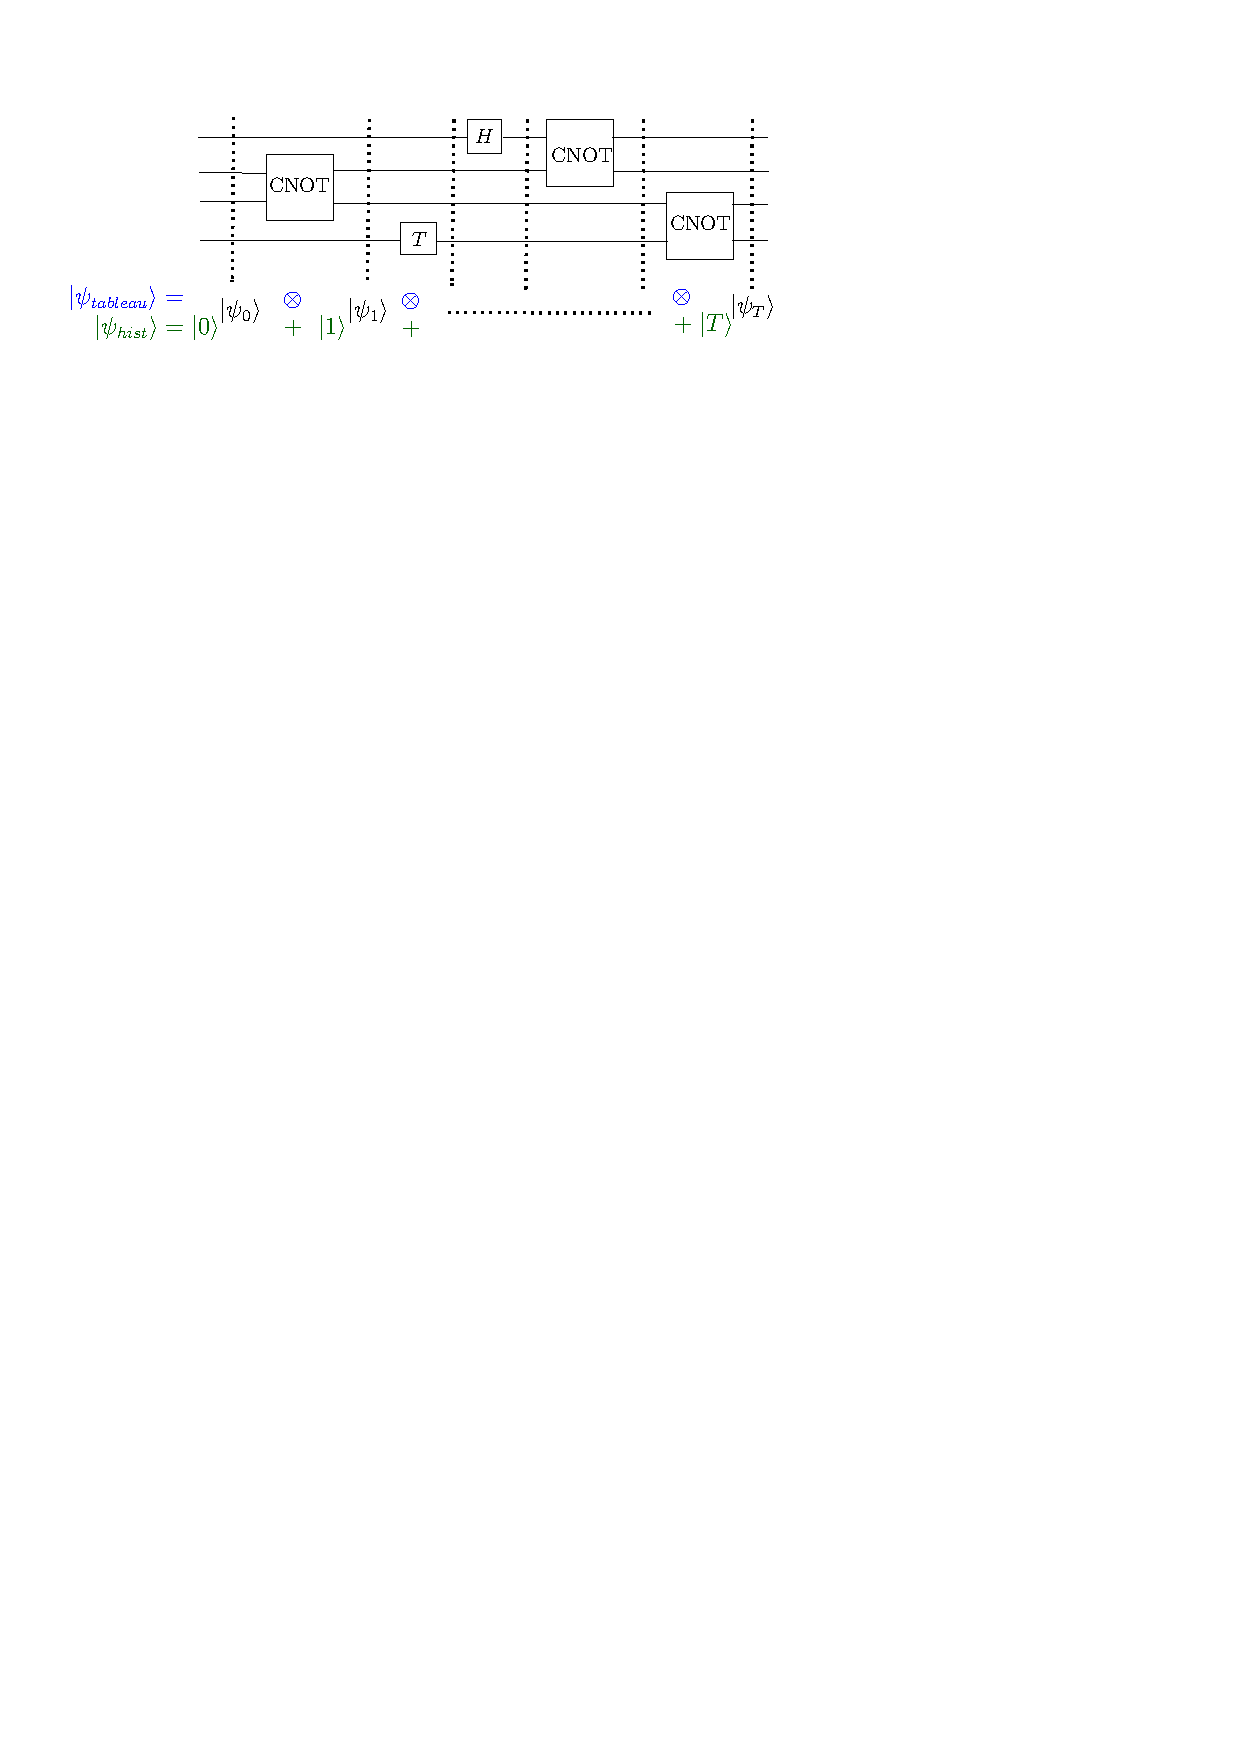
\includegraphics[scale=1, angle = 0]{qtableau.pdf}
%\hfill
\caption{Two different ways to create a tableau from a quantum circuit. The state $\ket{\psi_{tableau}}$ is the tensor product of the state of the circuit at each time step. The state $\ket{\psi_{hist}}$ is their superposition, indexed by a clock register that goes from $\ket{0}$ to $\ket{T}$.}
\label{fig:q-tableau}
\end{figure}


For quantum circuits the idea of a tableau of the computation is less straightforward. The most direct analogue is to consider the juxtaposition of the quantum state of a $T$-gate circuit at each step of the computation, i.e. the tensor product $\ket{\psi_0}\otimes \cdots\otimes \ket{\psi_T}$ of the states $\ket{\psi_i}$ obtained by executing the circuit from scratch and stopping after $i$ gates have been applied. While this is a well-defined $n(T+1)$-qubit quantum state (see Figure~\ref{fig:q-tableau}) the property of being a valid ``quantum tableau'' cannot be enforced using \emph{local} constraints! The reason is subtle, and has to do with the possible presence of entanglement at intermediate steps of the computation. Indeed, there are quantum states that are very different, in the sense that they are perfectly distinguishable by some \emph{global} observable, yet cannot be distinguished at all by any \emph{local} observable, that would act on at most, say, half the qubits. An example is given by the two $n$-qubit ``cat'' (named after the homonymous animal) states
\[ \ket{\psi_{\pm}} = \frac{1}{\sqrt{2}} \big( \ket{0\cdots 0} \pm \ket{1\cdots 1} \big)\;.\]
The two states $\ket{\psi_+}$ and $\ket{\psi_-}$ are easily seen to be orthogonal, so that they can be perfectly distinguished by a measurement. But it is an exercise to verify that for any observable that acts on at most $(n-1)$ of the $n$ qubits, both states give exactly the same expectation value. (Informally, this is because any measurement on a strict subset of the qubits of the state necessarily destroys the coherence; the only relevant information, the $\pm$ sign, is encoded ``globally'' and cannot be accessed locally.)
Note that this is a uniquely quantum phenomenon: if two classical strings of bits have each of their bits equal, one pair at a time, then the strings are ``globally'' identical. Not so for quantum states.

So na\"ive tableaus will not do. In the late 1990s Alexei Kitaev introduced a very powerful idea that provides a solution. Kitaev's idea is to replace the juxtaposition of snapshot states by their \emph{superposition} (see Figure~\ref{fig:q-tableau}). A special ancilla system, called the ``clock'', is introduced to index different elements of the superposition. Thus, instead of defining a tableau as $\ket{\psi_0} \cdots \ket{\psi_T}$, Kitaev considers the state
\begin{equation}\label{eq:h-state}
 \ket{\psi_{hist}}\,=\,\frac{1}{\sqrt{T+1}} \sum_{t=0}^T \ket{t}\ket{\psi_t}\;.
\end{equation}
Note that this takes less qubits to store, but this is not the important point. 
 Kitaev showed that, assuming the clock register is encoded in unary, it is possible to check the correct propagation of every step of the circuit directly on this superposition by only applying local observables: there is a set of observables $H_{in}$ that checks that $\ket{\psi_0}$ has the right format; a set of observables $H_{prop}$ that checks propagation of the circuit, and an observable $H_{out}$ that checks that the output qubit of the circuit is in the right state. (In addition, there is a term $H_{clock}$ that checks that the clock register is well-formed, i.e. contains the representation of an integer in unary. This can be done locally by penalizing configurations of the form ``$\cdots 10\cdots$''.) The key point that makes this possible is that, while equality of quantum states cannot be decided locally when the states are juxtaposed, it becomes possible when they are given in superposition. As an exercise, we can verify that a measurement of the first qubit of the state
\[ \ket{\psi_{SWAP}} \,=\, \frac{1}{\sqrt{2}}\big( \ket{0} \ket{\psi_0} + \ket{1}\ket{\psi_1}\big)\]
in the Hadamard basis $\{ \ket{+},\ket{-}\}$ returns the first outcome with probability exactly $\frac{1}{2}(1+|\bra{\psi_0}\psi_1\rangle|^2)$. 
With more work, replacing the use of gadgets in the classical Cook-Levin reduction by techniques from perturbation theory, it is possible to write the resulting observables as a linear combination of local terms that all take a particularly simple form. 
The result is the following theorem from~\cite{cubitt2016complexity}.

\begin{theorem}\label{thm:kitaev}
For any integer $n\geq 1$ there are $n'=\poly(n)$, $a=a(n)$ and $\delta \geq 1/\poly(n)$ such that the following holds. 
Given a $T$-gate quantum circuit $\mC = ((G_1,i_1,j_1),\ldots,(G_T,i_T,j_T))$ acting on $n$ qubits, such that $T=\poly(n)$, and an input $x$ for the circuit, there exist efficiently computable real weights $\{J_{ij},\, i,j\in\{1,\ldots,n'\}\}$ such that $|J_{ij}|\leq 1$ for all $i,j$ and moreover if
\begin{equation}\label{eq:lh-comp}
H_\mC \,=\, - \sum_{i,j}\; \frac{J_{ij}}{2}\,\big(\sigma_{X,i} \sigma_{X,j} + \sigma_{Z,i} \sigma_{Z,j}\big)\;,
\end{equation}
where $\sigma_{X,i}$ and $\sigma_{Z,j}$ denote single-qubit Pauli $X$ and $Z$ operators acting on the $i$-th and $j$-th qubit respectively, 
then:
\begin{itemize}
\item (Completeness) If the circuit $\mC$ accepts its input $x$ with probability at least $2/3$, then the smallest eigenvalue of $H_\mC$ is at most a;
\item (Soundness) If the circuit $\mC$ accepts its input $x$ with probability at most $1/3$, then the smallest eigenvalue of $H_\mC$ is at least $a + \delta$.
\end{itemize} 
\end{theorem}

\begin{remark}
It is possible to modify Theorem~\ref{thm:kitaev} so that the completeness and soundness statements specify that ``if there exists a state $\ket{\phi}$ such that $\mC$ accepts on input $(x,\ket{\phi})$ with probability at least $2/3$...'' and ``if there does not exist a state $\ket{\phi}$ such that $\mC$ accepts on input $(x,\ket{\phi})$ with probability greater than $1/3$...'' respectively. Thus, Theorem~\ref{thm:kitaev} can be adapted to show that the problem of estimating the minimal energy of a Hamiltonian of the form~\eqref{eq:lh-comp} is a QMA-complete problem. 
\end{remark}


Theorem~\ref{thm:kitaev} provides us with a roadmap for the verification of quantum circuits: it is sufficient to verify the \emph{existence} of a quantum state that yields certain statistics, when some of its qubits are measured in the computational ($\sigma_Z$ observable) or Hadamard ($\sigma_X$ observable) basis. The reason this can be considered progress is that we no longer need to check the time evolution of a quantum state under a quantum cicuit; it is sufficient to collect measurement statistics and estimate the ``energy'' $\bra{\psi}H\ket{\psi}$.  In particular, the theorem readily leads to a verification protocol in a model where the prover has a full quantum computer, and the verifier only has a limited quantum device --- namely, a one-qubit memory, together with the ability to measure the qubit using either the $\sigma_X$ or $\sigma_Z$ observables. 


\subsection{The protocol}
\label{sec:fm-protocol}

Such a verification protocol was introduced by Fitzsimons and Morimae and refined in a paper with Hadju\v{s}ek. The protocol is summarized in Figure~\ref{fig:fhm-protocol}. In the protocol, the prover is required to prepare a smallest eigenstate of the Hamiltonian $H_\mC$ given in~\eqref{eq:lh-comp}. While it may not be immediately obvious at the level of our description, it is possible to prepare such a ``history state''~\eqref{eq:h-state} by executing a quantum circuit that is only mildly more complex than the original circuit $\mC$. 

\begin{figure}[htbp]
\rule[1ex]{16.5cm}{0.5pt}\\
Let $\mC$ be a quantum circuit provided as input, and $H_\mC$ the $n$-qubit Hamiltonian obtained from $\mC$ as in~\eqref{eq:lh-comp}. 
\begin{enumerate}
\item The verifier initializes a counter $\gamma$ to $0$. She executes the following interaction with the prover independently $N=\frac{C}{\delta^2} {n' \choose 2}^2 \ln(1/\eps)$ times, where $C$ is a large enough universal constant:
\begin{enumerate}
\item The prover creates an eigenstate $\ket{\psi}$ of $H$ with smallest eigenvalue. 
\item The prover sends the qubits of $\ket{\psi}$ one by one to the verifier.
\item The verifier selects a measurement $W\in\{X,Z\}$ uniformly at random, and measures each qubit in the associated basis upon reception. Let $b_{W,i}\in\{-1,1\}$ be the outcome for the $i$-th qubit. 
\item The verifier selects $i\neq j \in \{1,\ldots,n'\}$ uniformly at random. She updates her counter $\gamma \leftarrow \gamma - J_{ij} b_{W,i} b_{W,j}$.
\end{enumerate}
\item If $\frac{\gamma}{N }{n' \choose 2} \leq a + \delta/2$ the verifier accepts the interaction. Otherwise, she rejects. 
\end{enumerate}
\rule[1ex]{16.5cm}{0.5pt}
\caption{The Fitzsimons-Hadju\v{c}ek-Morimae verification protocol, parametrized by a quantum circuit $\mC$ and an accuracy parameter $\eps>0$.}
\label{fig:fhm-protocol}
\end{figure}

We note that in the protocol, the verifier measures the qubits in a randomly chosen basis, and then selects a single pair $(i,j)$ such that $J_{ij}\neq 0$ uniformly at random to update her counter. One could imagine small optimizations where e.g.\ a maximum matching of such pairs is measured at each step. Such optimizations only bring marginal improvements in efficiency of the protocol; moreover they complicate the extension to a classical verifier that we will see later. For this reason, we prefer to keep the simplest expression possible for the protocol. 


\begin{theorem}\label{thm:fm}
Let $\mC$ be a quantum circuit and $H_\mC$ the Hamiltonian associated to it as in~\eqref{eq:lh-comp}. Let $x$ be an input to the circuit $\mC$ and $\eps>0$ a parameter for the protocol. Then the following hold:
\begin{itemize}
\item (Completeness:) If $\mC$ accepts $x$ with probability at least $2/3$, then there is a QPT prover that is accepted with probability at least $1-\eps$
\item (Soundness:) If $\mC$ accepts $x$ with probability at most $1/3$, then any prover is accepted with probability at most $\eps$. 
\end{itemize}
\end{theorem}

Note that in the theorem, the soundness statement does not place any computational assumption on the prover. 

\begin{proof}
The key calculation that underlies the proof is the following. 

\begin{claim}\label{claim:fm-1}
Let $\rho$ be the density matrix that represents the mixture over the $N$ $n'$-qubit states sent by the prover in the protocol (in general these states may be entangled). Then the expectation of $\gamma/N$ is exactly
\begin{equation}\label{eq:fm-eq-1}
\Es{} \Big[ \frac{\gamma}{N} \Big] \,=\, -\frac{1}{ {n' \choose 2}} \,\sum_{i\neq j}\, \frac{J_{ij}}{2} \,\Tr\big(\big(\sigma_X^i \sigma_X^j + \sigma_Z^i \sigma_Z^j\big)\rho\big)\,=\, \frac{1}{ {n' \choose 2}}\, \Tr\big(H\rho\big)\;.
\end{equation}
Moreover, for $N$ chosen as in the protocol for a large enough choice of the constant $C$ it holds that
\begin{equation}\label{eq:fm-eq-2}
\Pr\Big( \Big|\frac{\gamma}{N} {n'\choose 2} - \Tr\big(H\rho\big)\Big|> \frac{\delta}{2} \Big) \,\leq \,\eps\;.
\end{equation}
\end{claim} 

\begin{proof}
For $t\in\{1,\ldots,n\}$ let $G_t$ denote the product of the two outcomes $b_{W,i}$ and $b_{W,j}$ obtained by the verifier at step (c) of the protocol, where $W$, $i$ and $j$ are as sampled at step (d). Then the random variables $G_t \in \{-1,1\}$ are i.i.d. such that for each $t$, $\Es{}[G_t]= \Tr(\sigma_W^i \sigma_W^j \rho)$, with $W$, $i$ and $j$ are the values sampled in step $t$. Since $\gamma = - \sum_t J_{ij} G_t$, averaging over those choices gives~\eqref{eq:fm-eq-1}. Using $|J_{ij}|\leq 1$, by Hoeffding's inequality for any $s>0$
\[ \Pr\big( \big|\gamma - \Es{}[\gamma]\big| > s \big) \,\leq \, e^{-\frac{2  s^2 }{ 4N}}\;.\]
By choosing $N$ sufficiently large with respect to ${n' \choose 2}^2\delta^{-2}\ln(1/\eps)$ we get~\eqref{eq:fm-eq-2}.
\end{proof}

Based on Claim~\ref{claim:fm-1} the proof of Theorem~\ref{thm:fm} follows rather directly. For the completeness, we take $\rho = \proj{\psi}$ such that $\bra{\psi} H \ket{\psi} \leq a$, whose existence is guaranteed by the completeness case of Theorem~\ref{thm:kitaev}. As noted above, this $\rho$ can be prepared efficiently by a QPT prover. Using~\eqref{eq:fm-eq-2} it follows that this prover is accepted with probability at least $1-\eps$. For the soundness, $\rho$ is arbitrary. Using the soundness case of Theorem~\ref{thm:kitaev} it must be that $\Tr(H\rho) \geq a+\delta$, so that the conclusion follows again from~\eqref{eq:fm-eq-2}. 
\end{proof}




Even though the verifier's ``quantumness'' in this protocol is limited --- she only needs to hold one qubit at a time --- this capability is crucial for the analysis, as it is used to guarantee the ``existence'' of the state that is being measured: it allows us to meaningfully talk about ``the state $\rho$ whose first qubit is the first qubit received by the verifier; whose second qubit is the second qubit received by the verifier; etc.''. These qubits are distinct, because the verifier has seen and then discarded them (it would be a different matter if they were returned to the prover). In particular, the fact that a one-qubit computer can be trivially simulated on a classical piece of paper is immaterial to the argument.

With a classical verifier things become substantially more delicate. How can we verify the existence of an $n$-qubit state with certain properties, while having only access to classical data about the state, data that, for all we know a priori, could have been generated by a simple --- classical --- laptop? To achieve this we need to find a way for the verifier to establish that the prover holds an $n$-qubit state, without ever having the ability to directly probe even a single qubit of that state. In the previous lecture we saw a means to achieve this for a single qubit based on the computational hardness of certain functions called ``claw-free''. In the next lecture we extend that method to introduce a protocol by which the prover can certify the existence of any single-qubit state that is a low-energy eigenstate of a single-qubit Hamiltonian. In the last lecture we combine this extension with the Fizsimons-Morimae protocol to obtain a protocol for delegating quantum computations with a classical client. 

\chapter{Verifying a single qubit-Hamiltonian}

In the previous lecture we introduced the circuit-to-Hamiltonian construction, that given a quantum circuit $\mC$ and an input $x$ to it returns a Hamiltonian $H_\mC$ of the form~\eqref{eq:lh-comp} such that the completeness and soundness properties stated in Theorem~\ref{thm:kitaev} hold. This construction allowed us to reduce the problem of delegating a quantum computation to the problem of deciding if a certain publicly known, explicitly specified exponential-size Hermitian matrix $H_\mC$ has an eigenvalue below a certain threshold $a$, or all its eigenvalues are above $b+\delta$ for a $\delta$ that is at least inverse polynomial in the number of qubits $n$ on which $H_\mC$ acts.\footnote{In the previous lecture this number of qubits was called $n'$, with $n$ the number of qubits of the circuit $\mC$. For the next two lectures, $\mC$ disappears and so we re-use $n$ to measure the size of $H_\mC$.} We then introduced the Fitzsimons-Morimae protocol (Figure~\ref{fig:fhm-protocol}) that is a protocol with one-way communication for verifying this fact. 

Our goal in the next two lectures is to combine the Fitzsimons-Morimae protocol with the computational test for a qubit from lecture~\ref{chap:computational-test}, Section~\ref{sec:comp-test} to obtain a classical protocol with similar guarantees to the Fitzsimons-Morimae protocol. For this we will develop a test that allows one to verify that a prover ``has'' a quantum state $\ket{\psi}$ with certain properties (e.g.\ it satisfies $\bra{\psi}H\ket{\psi} \leq a + \delta/2$, i.e.\ certifies that the outcome of the computation is `$1$'. Note that even though in principle it is sufficient for the verifier to be convinced  that such a $\ket{\psi}$ exists to make the right decision, we will see from the proofs that we can go a little further and give a precise meaning to the notion that the prover `has' $\ket{\psi}$. This, however, will not be as strong as the claim that the prover `has $n$ qubits in state $\ket{\psi}$' in the sense that we gave to the phrase `has $n$ qubits', i.e.\ we will not quite exhibit $2n$ Pauli operators $X_i,Z_i$ that satisfy all the required relations. 


\begin{remark}
In passing to the Hamiltonian model of computation we relaxed our main goal,  from obtaining a value $b \in \{0,1\}$ that is distributed as a measurement of the output qubit of the quantum circuit $\mC$ in the standard basis to obtaining a value that is $1$ whenever this measurement returns $1$ with probability larger than $\frac{2}{3}$, and $0$ whenever it is less than $\frac{1}{3}$. In particular, we make no requirement for circuits that are ``undecided'', e.g. return a random bit as output. This is typical to applications in complexity where it is assumed that circuits of interest make a clear-cut decision, $0$ or $1$; this is the setting discussed in Section~\ref{sec:delegation-definitions}. By tweaking the definition of $H_\mC$ it is in fact possible to guarantee that any state $\ket{\psi}$ such that $\bra{\psi} H_\mC \ket{\psi} \leq a + \delta/2$ is such that a measurement of the first qubit of $\ket{\psi}$ in the standard basis yields an outcome whose distribution is within total variation distance, say, $\frac{1}{100}$ from a measurement of the output qubit of $\mC$. Using this observation the protocol given at the end of this lecture can be adapted to return outcomes that are distributed close to the circuit output distribution, even in cases where the output is not assumed to be biased one way or the other. For simplicity we leave this extension as an exercise to the reader. 
\end{remark}


\section{A test for a specific single-qubit Hamiltonian}

We start with an ``easy'' case: we show how the computational test for a qubit from lecture~\ref{chap:computational-test}, protocol~$\pq$, can be cast as a verification protocol for the claim that the Hamiltonian $H=-\sigma_Z$ has a ``low'' eigenvalue, equal to $-1$. We go a little further by showing how such an eigenstate can be ``extracted'' from any successful prover in the protocol. 

\subsection{An explicit isometry}
\label{sec:explicit-iso}

Our main result on the computational qubit test, Theorem~\ref{thm:comp-qubit}, states that any successful prover in the protocol must ``have a qubit''. The proof achieves slightly more than that, as it explicitly states what the observables $Z$ in~\eqref{eq:comp-qubit-proof-1a} and $X$ in~\eqref{eq:comp-qubit-proof-1b}  that define the qubit $(\ket{\psi},Z,X)$ are. As we saw in Lemma~\ref{lem:qubit-2-rigid} the qubit implies the existence of an isometry $V:\mH\to \C^2\otimes \mH'$ under which $Z\simeq \sigma_Z$, $X\simeq \sigma_Z$, and $\ket{\psi}\simeq \ket{\psi'} \in \C^2 \otimes \mH'$, giving us an identification of the ``abstract'' qubit $(\ket{\psi},Z,X)$ with a ``concrete'' qubit, i.e.\ the space $\C^2$ and its algebra of operators, of which $\sigma_Z$ and $\sigma_X$ form a linear basis. 

With our present goal of ``extracting'' a specific quantum state (a low-energy eigenstate for the Hamiltonian $H_\mC$) it is worthwhile making $V$ a little more explicit. Indeed, an important point that we did not emphasize so far is that this identification is not ``canonical''. The standard proof of Lemma~\ref{lem:qubit-2-rigid} involves an application of Jordan's lemma to identify a block structure such that in each block, $Z$ and $X$ act like $\sigma_Z$ and $\sigma_X$ respectively. These blocks are obtained by diagonalizing the operator $(X+Z)$. In the case where $X$ and $Z$ anti-commute this operator has only two eigenvalues, $\pm\sqrt{2}$, and the associated eigenspaces are highly degenerate. Any choice of a basis for one of the eigenspaces can be used to specify an isometry $V$ (a basis for the other eigenspace is determined by the first). (That there would be such a degeneracy is easily seen by observing that composing $V$ with any unitary on $\mH'$ still gives a valid isometry with the same properties.)

It is, in fact, possible to define a canonical choice for the isometry. This choice has the advantage that it is explicit and from a computational viewpoint leads to a circuit for $V$ that can be constructed from circuits for $X$ and $Z$. The idea behind the definition is to use the operators $X$ and $Z$ to ``teleport'' the abstract qubit $(\ket{\psi},Z,X)$ into a ``concrete'' qubit $(\ket{\varphi},\sigma_Z,\sigma_X)$ by means of an EPR pair. This is done in the following proposition. 

\begin{proposition}\label{prop:explicit-iso}
Let $(\ket{\psi},Z,X)$ be a qubit on $\mH$. Let $\ket{\phi^+} = \frac{1}{\sqrt{2}} (\ket{0}\ket{0} + \ket{1}\ket{1})\in \C^2 \otimes \C^2$ be the state of an EPR pair. Let $\mH'= \C^2_\reg{A} \otimes \mH$ and $V: \mH \to \C^2_\reg{Q} \otimes \mH'$ defined by
\begin{equation}\label{eq:explicit-isometry}
 \forall \ket{\varphi} \in \mH\;,\quad V\ket{\varphi} = \frac{1}{2}\big(\Id \otimes \Id_\reg{A}\otimes \Id_\reg{Q} + X \otimes \sigma_X \otimes \Id_\reg{Q} + Z \otimes \sigma_Z \otimes \Id_\reg{Q} + XZ \otimes \sigma_X\sigma_Z \otimes \Id_\reg{Q}\big) \ket{\varphi} \ket{\phi^+}_{\reg{AQ}}\;,
\end{equation}
where the systems in the range of $V$ are re-ordered so that the first factor $\C^2$ is associated with the second qubit of $\ket{\phi^+}_{\reg{AQ}}$ in~\eqref{eq:explicit-isometry}, and $\mH'$ consists of the state of the first qubit of $\ket{\phi^+}$, i.e.\ register $\reg{A}$, as well as the part of the state in $\mH$.  
Then $V$ is an isometry and for all $W\in\{X,Z\}$,
\begin{equation}\label{eq:explicit-isometry-2}
VW \ket{\psi}\, = (\sigma_W \otimes \Id) V \ket{\psi}\;.
\end{equation}
\end{proposition}

\begin{proof}
The proof is by direct calculation. First we verify that $V$ is indeed an isometry. This is simply because the four states $\{(\sigma_X(a)\sigma_Z(b) \otimes \Id)\ket{\phi^+},\, a,b\in\{0,1\}\}$ are orthonormal\footnote{For $a,b\in\{0,1\}$ we use the notation $\sigma_X(a)$ for $\sigma_X^a$ and similarly $\sigma_Z(b)$ for $\sigma_Z^b$. The motivation for this notation will be seen later when we consider $n$-qubit Pauli operators.} and $X$ and $Z$ are observables, so that for normalized $\ket{\varphi}$ each of the four terms on the right-hand side of~\eqref{eq:explicit-isometry} has norm exactly $1$. Note that this does not require any other condition on $X,Z$ than that they are observables (in fact, unitarity suffices). In particular, they do not need to anti-commute. Next we verify~\eqref{eq:explicit-isometry-2}. 
Take $W=X$. Then
\begin{align*}
 VX \ket{\psi} &= \frac{1}{2}\big(X \otimes \Id\otimes \Id + \Id \otimes \sigma_X \otimes \Id -XZ \otimes \sigma_Z \otimes \Id -Z \otimes \sigma_X\sigma_Z \otimes \Id\big) \ket{\psi} \ket{\phi^+} \\
&= \frac{1}{2}\big(X \otimes \Id\otimes \Id + \Id \otimes \sigma_X \otimes \Id -XZ \otimes \sigma_Z \otimes \Id -Z \otimes \sigma_X\sigma_Z \otimes \Id\big) \ket{\psi} (\sigma_X \otimes \sigma_X)\ket{\phi^+} \\
&= \frac{1}{2}\big(X \otimes \sigma_X \otimes \sigma_X + \Id \otimes \Id \otimes\sigma_X +XZ \otimes \sigma_X \sigma_Z \otimes \sigma_X +Z \otimes \sigma_Z \otimes \sigma_X\big) \ket{\psi} \ket{\phi^+} \\
&= (\sigma_X \otimes \Id) V \ket{\psi}\;,
\end{align*}
where for the first line we used that $X$ and $Z$ anti-commute on $\ket{\psi}$, for the second that $\sigma_X\otimes \sigma_X \ket{\phi^+} = \ket{\phi^+}$, for the third that $\sigma_X$ and $\sigma_Z$ anti-commute, and for the last we re-ordered terms. 
\end{proof} 

\subsection{Extraction of prover's qubit}
\label{sec:extract-simple}

In the proof of Theorem~\ref{thm:comp-qubit} we defined a specific $X$ and $Z$ from the prover's actions and showed that they anti-commute. Moreover, we showed that for a prover that always succeeds in the equation test (case $c=1$) it must be the case that the state $\ket{\psi}$ of the prover is a $+1$ eigenstate of $X$, $X\ket{\psi}=\ket{\psi}$. For the definition of $\ket{\psi}\in\mH_\reg{X}\otimes \mH_\reg{P}$, recall that we had assumed that the prover directly measures the qubits in register $\reg{X}$ on challenge $c=0$, and applies an arbitrary unitary $U$ before measuring in the Hadamard basis on challenge $c=1$. This means that after the isometry $V$, the prover's state $\ket{\psi}$ is mapped to a $+1$ eigenstate of $\sigma_X$, i.e.\ the state $\ket{+}$. The following corollary summarizes this discussion. 

\begin{corollary}\label{cor:comp-qubit}
Suppose that a prover succeeds with probability $1$ in the protocol. Then the isometry $V$ defined from the observables  $Z$ in~\eqref{eq:comp-qubit-proof-1a} and $X$ in~\eqref{eq:comp-qubit-proof-1b} sends $\ket{\psi}$ to $\ket{+}_\reg{Q}\ket{aux}$, for some state $\ket{aux}$ on $\mH'$.
\end{corollary}

In the context of this lecture we interpret Corollary~\ref{cor:comp-qubit} as our first test for a quantum computation in the Hamiltonian-based model: in this test, the verifier is effectively checking that the prover has prepared a $+1$ eigenstate of the Hamiltonian $\sigma_X$, or in other words a ground state of $H=-\sigma_X$. While we know that this eigenstate always exists, the analysis of the protocol shows that in some sense the prover has prepared the state. This additional observation allows us to make stronger conclusions from the protocol. For example, just as a measurement of $\ket{+}$ in the computational basis yields an unbiased random bit, we are able to deduce that the value of $b(x)$ with $x$ the prover's answer on challenge $c=0$ is an unbiased random bit. This makes the protocol potentially useful for cryptographic applications where the generation of certified unbiased randomness serves as a resource.  

In the development of our test we were greatly aided by the fact that we \emph{know} what is the ground state of $H = -\sigma_X$, and in particular we know that a Hadamard basis measurement of it yields the outcome $0$ (for `$+$') with probability $1$. This ``knowledge'' was indirectly encapsulated in the test performed for the case $c=1$, the analysis of which led us to conclude that $X \ket{\psi} = + \ket{\psi}$. 
But what if we didn't? What if $H$ is a general Hamiltonian of the form~\eqref{eq:lh-comp}, for which we can't a priori predict measurement outcomes? 


\section{Extracting a qubit: general case}
\label{sec:extract-comp-qubit}

In Section~\ref{sec:explicit-iso} we made the important observation that the map $V$ in~\eqref{eq:explicit-isometry} is a well-defined isometry for any choice of the two observables $X$ and $Z$. In particular, this map allows us to make a meaningful definition of a \emph{space} for a qubit, and a \emph{state} for that qubit, associated with \emph{any} prover in protocol $\pq$, the computational test for a qubit described in Figure~\ref{fig:protocol-comp-test}. This definition does not guarantee that the prover ``has a qubit,'' because it does not say anything about how the prover's observables operate on it. 
 However, it still allows us to define a \emph{candidate} for a single-qubit state on which $\sigma_X$ and $\sigma_Z$ measurements can \emph{in principle} be made. The next claim evaluates how outcomes of these measurements when performed on the extracted qubit are distributed as a function of the observables $X$ and $Z$ on the prover's state $\ket{\psi}$. 

\begin{claim}\label{claim:iso-xz}
Let $\ket{\psi} \in \mH$ and $X,Z$ observables on $\mH$ be arbitrary. Let $V$ be defined as in~\eqref{eq:explicit-isometry}. Then the following hold:
\begin{align}
\bra{\psi} V^\dagger \big(\sigma_Z \otimes \Id\big) V \ket{\psi} &= \bra{\psi} Z \ket{\psi}\;,\label{eq:isometry-z}\\
\bra{\psi} V^\dagger \big(\sigma_X \otimes \Id\big) V \ket{\psi} &= \frac{1}{2} \big(  \bra{\psi} X \ket{\psi} -  \bra{\psi} ZXZ \ket{\psi} \big)\;,\label{eq:isometry-x}
\end{align}
where the $\sigma_Z$ and $\sigma_X$ operators act on the first tensor factor $\C^2$ in the range of $V$ and the identities act on $\mH'$. 
\end{claim}

Recalling the diagram~\ref{diag:one-qubit} introduced to illustrate Lemma~\ref{lem:qubit-2-rigid}, Claim~\ref{claim:iso-xz} can similarly be illustrated as follows, where $\Es{b}$ denotes the average over $b$:
\begin{equation}\label{diag:one-qubit-b}
\begin{tikzcd}
\mH  \arrow{r}{V}  \arrow[swap]{dd}{\substack{Z \\[3mm] \Es{b\in\{0,1\}} (-1)^b\, Z^bXZ^b }} &  \C^2 \otimes \mH' \arrow{dd}{\substack{\sigma_Z\otimes \Id\\[3mm] \sigma_X\otimes \Id}} \\
&\\ 
\mH  \arrow{r}{V} & \C^2 \otimes \mH'
\end{tikzcd}
\end{equation}
We emphasize that this diagram is purely illustrative and should be understood exactly in the sense of~\eqref{eq:isometry-z} and~\eqref{eq:isometry-x}; i.e.\ it does not imply a relation on the operators but only on the expectation values on the state $\ket{\psi}$. Informally, when considering expectation values only the isometry has the effect of applying a $Z$-twirl to the Hadamard basis observable $X$. 

\begin{proof}
Let $W\in\{X,Z\}$. Expanding from the definition of $V$,
\begin{align*}
\bra{\psi} V^\dagger \big(\sigma_W \otimes \Id\big) V \ket{\psi}
&= \frac{1}{4}\sum_{P,Q\in \{I,X,Z,XZ\}} \,\bra{\psi} P^\dagger Q \ket{\psi}\cdot \bra{\phi^+} \sigma_P^\dagger \sigma_Q \otimes \sigma_W \ket{\psi}\\
&= \frac{1}{4}\sum_{P,Q:\, \sigma_P^\dagger \sigma_Q = \sigma_W} \,\bra{\psi} P^\dagger Q \ket{\psi}\;,
\end{align*}
where for the second line we used that $\bra{\phi^+} \sigma_W \otimes \sigma_{W'} \ket{\phi^+} = \delta_{W,W'}$ with $\delta$ the Kronecker symbol. In case $W=Z$ the pairs $P,Q$ that appear in the last summation above are $(X,I),(I,X),(XZ,X)$ and $(X,XZ)$. Using $X^2 = \Id$ we obtain~\eqref{eq:isometry-z}. In case $W=X$ then the summation is over $(Z,I),(I,Z),(XZ,Z)$ and $(Z,XZ)$ and has a minus sign for the last two terms due to $\sigma_X\sigma_Z = -\sigma_Z\sigma_X$. Thus we get~\eqref{eq:isometry-x} as well. 
\end{proof}

Observe that if $X$ and $Z$ anti-commute then Claim~\ref{claim:iso-xz} gives us the result that we expect: in this case $(\ket{\psi},Z,X)$ is a qubit so Proposition~\ref{prop:explicit-iso} applies and the isometry ``intertwines'' measurements $X$ and $Z$ on $\ket{\psi}$ with $\sigma_X$ and $\sigma_Z$ respectively on the first factor of $V\ket{\psi}$. At the other extreme, if $X$ and $Z$ commute then~\eqref{eq:isometry-x} indicates that a measurement in the Hadamard basis of the extracted qubit returns an unbiased random bit. This is expected of a ``classical'' state, which always leads to uniformly random results in the Hadamard basis. The lemma in some sense interpolates between these results. Importantly, it allows us to associate a qubit with the state of an arbitrary prover in the protocol, that is such that the distribution of measurements on the extracted qubit can be related to  quantities that involve the prover's state and observables in the protocol. For convenience we make this into a definition. 

\begin{definition}[Extracted qubit]\label{def:extracted-qubit}
Let $P$ be a prover in protocol~$\pq$. Let $\ket{\psi}$ be the state of $P$ after having sent $y$ in the first round of interaction. Let $V$ be defined as in~\eqref{eq:explicit-isometry}. Then we call the reduced density of $V\ket{\psi}$ on the first factor $\C^2$, associated with register $\reg{Q}$, the \emph{extracted qubit} and denote it by $\rho_\reg{Q}$. 
\end{definition}

\begin{lemma}\label{lem:comp-ind-qubits}
Let $P$ be a prover that succeeds with probability $1$ in the pre-image test of  protocol~$\pq$ and such that the string $d$ returned in the equation test is $d=0^m$ with probability that is negligibly small in $\lambda$. (No other assumption is made on the equation test.) Let $\rho$ be the extracted qubit, as defined in Definition~\ref{def:extracted-qubit}. Then the following hold:
\begin{itemize}
\item ($Z$-measurement:) The outcome of measuring $\rho$ in the computational basis is identically distributed to the bit $(-1)^{b(x)}$ computed from the prover's answer $x$ in case $c=0$.
\item ($X$-measurement:) Under assumption~\ref{ass:f2}, the outcome of measuring $\rho$ in the Hadamard basis is \emph{computationally indistinguishable} from the bit $(-1)^{d\cdot(x_0+x_1)}$ where $d$ is obtained from the prover in case $c=1$.
\end{itemize}
\end{lemma}

\begin{remark}[Computational distinguishability]\label{rk:comp-dist}
The statement of the lemma refers to two distributions being computationally indistinguishable. Informally, this means that no computationally efficient procedure can distinguish a sample taken from one distribution from a sample taken from the other. Formally, families of distributions $D = \{D_\lambda\}$ and $D' = \{D'_\lambda\}$ on universes $\{\mX_\lambda\}$ are said to be  computationally indistinguishable if for any PPT (or QPT for computational indistinguishability against quantum adversaries) procedure $\mA$ there is a negligible function $\mu$ such that for every $\lambda$,
\[ \Big|\Pr_{x\leftarrow D_\lambda}\big( \mA(1^\lambda,x)=1\big) - \Pr_{x' \leftarrow D'_\lambda}\big(\mA(1^\lambda,x')=1\big)\Big|\,\leq\, \mu(\lambda)\;.\]
Here, when we refer to computational indistinguishability we will always mean against QPT adversaries. Note that for distributions on a family of universes $\{\mX_\lambda\}$ such that $|\mX_\lambda|$ grows at most polynomially with $\lambda$ the notion of computational indistinguishability is equivalent to statistical indistinguishability, i.e.\ the total variation distance between $D_\lambda$ and $D'_\lambda$ goes to $0$ as fast as some negligible function. (Showing this formally is a good exercise to practice with the definitions.)
\end{remark}



\begin{proof}
The first item follows immediately from~\eqref{eq:isometry-z} in Claim~\ref{claim:iso-xz} and the definition of $Z$ in~\eqref{eq:comp-qubit-proof-1a}, which guarantees that  the bit $(-1)^{b(x)}$ obtained from the prover in case $c=0$ has expectation precisely $\bra{\psi} Z \ket{\psi}$. 

To show the second item we assume for contradiction that the two distributions are computationally distinguishable. Since the distributions are over a single bit, as recalled in Remark~\ref{rk:comp-dist} this is equivalent to statistical distinguishability: there must exist a polynomial $q(\lambda)$ such that for infinitely many values of $\lambda$, 
\begin{equation}\label{eq:comp-ind-qubits-1}
 \big|\bra{\psi} X \ket{\psi} +  \bra{\psi} ZXZ \ket{\psi}\big| \,>\, \frac{1}{q(\lambda)}\;,
\end{equation}
where recall that the expression on the left should be understood on average over the generation of $pk$ by the verifier and the message $y$ sent by the prover in the first round of interaction. We derive a contradiction with~\ref{ass:f2} by constructing an adversary in~\eqref{eq:hc-bit-0}.  Given $\lambda$ and $pk$ as input, $\mA$ prepares the state $\ket{\psi}$. $\mA$ then measures register $\reg{X}$ in the standard basis to obtain an outcome $x$. Using the assumption that the prover succeeds with probability $1$ in the pre-image test, $f_{pk}(x)=y$ and the (unnormalized) post-measurement state is exactly $Z_{b(x)}\ket{\psi}$, where as usual $Z_b = (\Id + (-1)^b Z)/2$.  Finally, the adversary applies the prover's unitary $U$ and measures in the Hadamard basis to obtain a string $d$. It returns the pair $(x,d)$. The expected value of $(-1)^{d\cdot (x_0+x_1)}$ under this procedure is 
\[ \bra{\psi} Z_0 X Z_0 \ket{\psi} + \bra{\psi} Z_1 X Z_1 \ket{\psi} \,=\,\frac{1}{2}\big(\bra{\psi} X \ket{\psi} +  \bra{\psi} ZXZ \ket{\psi}\big)\;,\]
which can be seen by expanding $Z_b=(\Id+(-1)^b Z)/2$ for $b\in \{0,1\}$ and canceling cross-terms. Using~\eqref{eq:comp-ind-qubits-1} and the fact that, $\mA$ violates~\eqref{eq:hc-bit-0}.\footnote{The end of the proof glosses over a detail: one needs to guarantee that the equation $d$ returned by $\mA$ is not $0$. While the lemma assumes that this is the case when the equation is measured directly on $\ket{\psi}$, here $\mA$ measures after $\ket{\psi}$ has already been measured using the observable $Z$. To show that the assumption that $d\neq 0^m$ with probability negligibly close to $1$ still holds one needs to use the ``collapsing'' property of $f_{pk}$, that we will introduce in the next lecture.}
\end{proof}


\section{A single-qubit verification protocol}

In the previous section we showed how to identify a ``qubit'' such that for any prover in the protocol, as long as the prover succeeds in the preimage test then it is possible for the verifier to infer from the prover's answers a bit whose distribution is statistically indistinguishable from outcomes of $\sigma_Z$ or $\sigma_X$ measurements on a well-defined quantum state. In order to turn this into a verification protocol for a single-qubit Hamiltonian, we are missing the completeness statement: while in Section~\ref{sec:comp-test} we saw how a prover could behave in such a way that the extracted qubit is a $\ket{+}$ state, we do not yet know if it is possible to use the protocol for the verification of other single-qubit states. In order for this to work out, we make the following assumption that replaces assumption~\ref{ass:f4}:
\begin{enumerate}[label=(\textbf{F.4'})]
\item\label{ass:f4b} For any $pk$ and any $y$ in the range of $f_{pk}$ the two preimages of $y$ take the form $(b,x_b)$ where $b\in\{0,1\}$ and $x_b \in \{0,1\}^{m(\lambda)-1}$. In particular, the function $b:\{0,1\}^m \to \{0,1\}$ returns the first bit of its input. 
\end{enumerate}
This assumption is mainly for convenience and holds for most constructions of claw-free functions, including the one that we sketch in the next lecture. Given a $2$-to-$1$ function family that satisfies~\ref{ass:f4b} the following lemma shows how a prover can behave in the protocol so that the extracted qubit defined in the previous section is a state $\ket{\varphi}$ of its choice. 

\begin{lemma}\label{lem:oq-completeness}
Let $\ket{\varphi}\in\C^2$ be any state. Then there is a way for the prover to behave in protocol~$\pq$ such that the prover is accepted with probability $1$ in the preimage test and moreover the extracted qubit satisfies $\rho_\reg{Q} = \proj{\varphi}$. 
\end{lemma}

\begin{proof}
Let $\ket{\varphi} = \alpha\ket{0} + \beta \ket{1}$ for $\alpha,\beta\in\C$ such that $|\alpha|^2 + |\beta|^2 =1$. The prover performs the following steps:
\begin{enumerate}
\item Prepare the initial state 
\[ \ket{\psi^{(0)}}_{\reg{BXY}} \,=\, \ket{\varphi}_\reg{B}\otimes \Big(\frac{1}{2^{m-1}} \sum_{x\in\{0,1\}^{m-1}} \ket{x}_{\reg{X}}\Big) \ket{0}_{\reg{Y}}\;,\]
where $\reg{B}$ is a one-qubit register, $\reg{X}$ an $(m-1)$ and $\reg{Y}$ an $m$-qubit register, for $m=m(\lambda)$. 
\item Upon receipt of the function index $pk$, coherently evaluate $f_{pk}$ on the input in registers $\reg{BX}$, writing the output in register $\reg{Y}$ to obtain the state
\[ \ket{\psi^{(1)}}_{\reg{BXY}} \,=\,  \frac{\alpha}{2^{m-1}}\sum_{x\in\{0,1\}^{m-1}} \ket{0}_\reg{B}\ket{x}_\reg{X}\ket{f(0x)}_\reg{Y} +  \frac{\beta }{2^{m-1}}\sum_{x\in\{0,1\}^{m-1}} \ket{1}_\reg{B}\ket{x}_\reg{X}\ket{f(1x)}_\reg{Y} \;.\]
\item Measure the last register to obtain a $y$. Let $(0,x_0)$ and $(1,x_1)$ be the two preimages of $y$ under $f_{pk}$. Then the re-normalized post-measurement state is
\[ \ket{\psi^{(2)}}_{\reg{BXY}} \,=\, \big(\alpha \ket{0}_\reg{B}\ket{x_0}_\reg{X} + \beta \ket{1}_\reg{B}\ket{x_1}_\reg{X}\big)\ket{y}_\reg{Y} \;.\]
\item Upon receipt of challenge $c$, perform as the honest prover in protocol $\pq$: if $c=0$ measure registers $\reg{BX}$ in the standard basis and return the outcome $x=(b,x_b)$; if $c=1$ measure in the Hadamard basis and return the outcome $d$.
\end{enumerate}
This prover always returns a valid preimage in the case of a challenge $c=0$, so it is accepted with probability $1$. Observe that the operator $Z$ associated to this prover is equal to a $\sigma_Z$ on register $\reg{B}$. Regarding the operator $X$, a simple calculation reveals that the action of $X$ restricted to the span of $\ket{0,x_0}_{\reg{BX}}$ and $\ket{1,x_1}_{\reg{BX}}$ consists in exchanging these two basis states. Using the explicit form of the isometry $V$ given in~\eqref{eq:explicit-isometry} one can verify that 
\[ V \ket{\psi^{(2)}} = \frac{1}{\sqrt{2}}\big(\ket{0}_\reg{B} \ket{x_0}_\reg{X} \ket{0}_\reg{A} + \ket{1}_\reg{B} \ket{x_1}_\reg{X} \ket{1}_\reg{A}\big) \otimes \big(\alpha\ket{0}_\reg{Q} + \beta\ket{1}_{\reg{Q}} \big)\otimes \ket{y}_\reg{Y}\;,\]
where $\reg{AQ}$ are the two registers introduced to hold the EPR pair $\ket{\phi^+}_{\reg{AQ}}$ used in the definition of $V$. Register $\reg{Q}$ contains the extracted qubit. 
\end{proof}


\begin{figure}[htbp]
\rule[1ex]{16.5cm}{0.5pt}\\
Let $\mF$ be a $2$-to-$1$ trapdoor claw-free function family and $\lambda\in\mathbb{N}$ a security parameter. Let $\eps,\delta>0$ be accuracy parameters.  Let $\gamma = 0$ and $N = \frac{C}{\delta^2} \ln(1/\eps)$ for some large constant $C$.
The verifier and prover repeat the following interaction $N$ times.
 \begin{enumerate}
\item The verifier generates $(pk,td)\leftarrow \textsc{Gen}(1^\lambda)$. It sends $pk$ to the prover. 
\item The prover returns $y \in \{0,1\}^m$, where $m=m(\lambda)$. 
\item The verifier selects a uniformly random challenge $c\leftarrow_R \{0,1\}$ and sends $c$ to the prover. 
\item 
\begin{enumerate}
\item \emph{(Computational basis, $c=0$:)} In case $c=0$ the prover is expected to return an $x\in\{0,1\}^m$. If $f(x)\neq 0$ then the verifier immediately aborts. The verifier sets $a\leftarrow (-1)^{b(x)}$ and $\gamma \leftarrow \gamma - J_Z a$. 
\item \emph{(Hadamard basis, $c=1$:)} In case $c=1$ the prover is expected to return a $d\in \{0,1\}^m$. The verifier uses $td$ to determine the two preimages $(x_0,x_1)$ of $y$ by $f_{pk}$. She sets $b\leftarrow (-1)^{d\cdot(x_0+ x_1)}$ and $\gamma \leftarrow \gamma - J_X b$. 
\end{enumerate}
\end{enumerate}
If the verifier has not aborted at any of the steps $c=0$, she returns the real number $o=\frac{1}{N}\gamma$. 
\rule[1ex]{16.5cm}{0.5pt}
\caption{Verification protocol for a single-qubit Hamiltonian $H = -\frac{J_X}{2} \sigma_X - \frac{J_Z}{2}\sigma_Z$.}
\label{fig:protocol-mahadev-oq}
\end{figure}

The following proposition summarizes what we have achieved so far, a verification protocol for single-qubit Hamiltonians and a completely classical verifier. (Of course a simpler protocol would be to have the verifier classically do the computation themselves! The point is that this protocol is not too hard to extend to $n$ qubits, as we will see in the next lecture.) The protocol, which combines protocol $\pq$ with the Fitzsimons-Morimae verification protocol, is summarized in Figure~\ref{fig:protocol-mahadev-oq}. 

\begin{proposition}\label{prop:mahadev-oq}
Let $H = -\frac{J_X}{2} \sigma_X -\frac{ J_Z}{2}\sigma_Z$ be a single-qubit Hamiltonian and $\delta,\eps>0$ accuracy parameters. Then the verification protocol from Figure~\ref{fig:protocol-mahadev-oq} has the following properties:
\begin{enumerate}
\item (Completeness:) For any single-qubit state $\ket{\varphi}$, there is a QPT prover that is accepted with probability $1$ in the protocol and such that the value $o$ returned by the verifier at the end of the protocol satisfies $\Es{}[o] = \bra{\varphi} H \ket{\varphi}$.
\item (Soundness:) For any QPT prover that is accepted with probability  $1$ in the protocol, there is a single-qubit state $\rho$ such that the value $o$ returned by the verifier at the end of the protocol satisfies $\Es{}[o] = \Tr(H\rho)$. 
\end{enumerate}
Moreover, with the value of $N$ specified in the protocol in both cases it holds that $\Pr(|o-\Tr(H\rho)| > \delta)\leq \eps$.
\end{proposition}

\begin{remark}\label{rk:prover-1}
The assumption that the prover succeeds with probability negligibly close to $1$ in the protocol can be relaxed to a constant sufficiently close to $1$, where the distance to $1$ will affect the distance $|\Es{}[{o}] - \Tr(H\rho)|$. First we observe that a success probability negligibly close to $1$ is sufficient; this can be verified by going through the argument again, and nothing needs to be changed. Second, it is possible to show that any prover with success probability $1-\kappa$ for some $\kappa \geq 0$ can be transformed to a prover with success probability negligibly close to $1$, affecting the distribution of $o$ proportionately to $\kappa$. Intuitively, the new prover will test if the value $y$ that the old prover would have returned will lead to success on challenge $c=0$, in case that the test is actually executed by the verifier. This can be done efficiently by the prover by evaluating the pre-image condition on register $\reg{X}$. If this test fails then the new prover simply re-executes the old prover from scratch, until it is certain to achieve success. With probability negligibly close to $1$ this iterative procedure will stop in a polynomial number of steps, and using the ``pretty-good lemma'' it is possible to show that the prover's distribution of outcomes is affected by some $O(\sqrt{\kappa})$ in statistical distance. We omit the details. 
\end{remark}

\begin{proof}
The completeness statement follows from Lemma~\ref{lem:oq-completeness}. For soundness we use Lemma~\ref{lem:comp-ind-qubits}. This shows that the expectation of the bit $a$ in step 4.(a) satisfies $\Es{} [a] =  \Tr(\sigma_Z \rho)$ where $\rho$ is the extracted qubit. Similarly, the bit $b$ in step 4.(b) satisfies $\Es{} [b] =  \Tr(\sigma_Z \rho)$. Since by definition
\[\Es{} [o] \,=\, -\frac{J_Z}{2}\, \Es{} [a] - \frac{J_X}{2}\, \Es{} [b] \]
the proposition follows. 
\end{proof}



\include{Lecture7b}


\bibliography{fsmp}

\end{document}




